\documentclass[10pt]{article}
\usepackage[utf8x]{inputenc}
\usepackage{amssymb, amsmath, amsfonts, amsthm, wasysym} % math
\usepackage{nicefrac}
\usepackage{geometry}
\usepackage{epsfig, subfigure} % graphics
%\usepackage[mathcal]{euscript}
\geometry{ top=2.5cm, bottom=2cm, left=2cm, right=2cm}
\usepackage[authoryear]{natbib}
\usepackage{pdflscape}
%\geometry{papersize={216mm,330mm}, top=3cm, bottom=2.5cm, left=4cm,  right=2cm}

\newcommand{\D}{\partial}
\newcommand{\Diff}[2] {\dfrac{\partial( #1)}{\partial #2}}
\newcommand{\diff}[2] {\dfrac{\partial #1}{\partial #2}}
\newcommand{\bv}[1]{\ensuremath{\mbox{\boldmath$ #1 $}}}
\newcommand{\gv}[1]{\ensuremath{\mbox{\boldmath$ #1 $}}}% for vectors of Greek letters
\newcommand{\grad}[1]{\gv{\nabla} #1}
\newcommand{\Rho}{\,\mathtt{Rho}}
%\newcommand{\PP}{\,\mathtt{P}}
\newcommand{\U}{\,\mathtt{U}}
\newcommand{\V}{\,\mathtt{V}}
\newcommand{\Nu}{\,\mathtt{Nu_{sa}}}
\newcommand{\T}{\,\mathtt{T}}
\newcommand{\Mu}{\,\mathtt{Mu}}
\newcommand{\Lo}{\,\mathcal{L}}
\newcommand{\Dueqplusyplus}{\, \frac{du_{eq}^+}{dy^+}\,}

% commands I like
\newcommand{\mbb}[1]{\mathbb{#1}}
\newcommand{\mbf}[1]{\mathbf{#1}}
\newcommand{\sbf}[1]{\boldsymbol{#1}}
\newcommand{\mcal}[1]{\mathcal{#1}}
\newcommand{\mfk}[1]{\mathfrak{#1}}
\newcommand{\pp}[2]{\frac{\partial #1}{\partial #2}}
\newcommand{\dd}[2]{\frac{d #1}{d #2}}
\newcommand{\rarrow}{\rightarrow}
\newcommand{\Rarrow}{\Rightarrow}
\newcommand{\LRarrow}{\Leftrightarrow}
\newcommand{\jump}[1]{\llbracket #1 \rrbracket}
\newcommand{\avg}[1]{\{ #1 \}}
\def\etal{{\it et al.~}}
\newcommand{\vvvert}{|\kern-1pt|\kern-1pt|}
\newcommand{\enorm}[1]{\vvvert #1 \vvvert}
\newcommand{\ud}{\,\mathrm{d}}

\newcommand{\sa}{\nu_{\mathrm{sa}}}
\newcommand{\tsa}{\mathrm{sa}}
\newcommand{\brho}{\bar{\rho}}
\newcommand{\bp}{\bar{p}}
\newcommand{\bq}{\bar{q}}
\newcommand{\tu}{\tilde{u}}
\newcommand{\tv}{\tilde{v}}
\newcommand{\tS}{\tilde{S}}
\newcommand{\tE}{\tilde{E}}
\newcommand{\bmu}{\bar{\mu}}
\newcommand{\hh}{\tilde{h}}
%opening
\title{Manufactured Solution for the 2D steady Favre--Averaged Navier--Stokes Equations with Spalart--Allmaras turbulence model}

\author{Kemelli C. Estacio-Hiroms$^*$ \\ Todd Oliver\thanks{Center for Predictive Engineering and Computational Sciences (PECOS), Institute for Computational
    Engineering and Sciences, The University of Texas at Austin,
    Austin, TX 78712 (\{kemelli,oliver\}@ices.utexas.edu)}}

\begin{document}

\maketitle
\tableofcontents

\begin{abstract}
The Method of Manufactured Solutions is a valuable approach for code verification, providing means to verify how accurately the numerical method solves the partial differential equations of interest.
This document presents the source terms generated by the application of the Method of Manufactured Solutions on the 2D steady Favre--Averaged Navier--Stokes Equations with Spalart--Allmaras turbulence model using analytical manufactured solutions that  reasonably resemble the inner portion (viscous sublayer and logarithmic layer) of a zero pressure gradient boundary layer.
\end{abstract}





\section{Mathematical Model}

%-------------------------------------------------
Turbulent flows occur at high Reynolds numbers, when the inertia of the fluid overwhelms the viscosity of the fluid, causing the laminar flow motions to become unstable. Under these conditions, the flow is characterized by rapid fluctuations in pressure and velocity which are inherently three dimensional and unsteady. Turbulent flow is composed of large eddies that migrate across the flow generating smaller eddies as they go. These smaller eddies in turn generates smaller eddies until they become small enough that their energy is dissipated due to the presence of molecular viscosity.

In practice, the effect of this sensitivity
is to make the value of any flow quantity at any particular point in
time and space uncertain.  Thus, these quantities may be viewed as
random variables with associated probability density functions,
allowing the use of statistical techniques in the description and
analysis of the flow. Or, in other words, the full influence of the turbulent fluctuations on the mean flow must be modeled.

For flows with significant density variations it is possible to  capture the turbulent effects using the Favre averaged Navier-Stokes equations (FANS), together with baseline compressible Spalart--Allmaras (SA) turbulent model~\citep{Oliver2010,Spalart_1994_One_Eqn_Turb_Model}.

Mass conservation:
\begin{equation}\label{eq:ns01}
\pp{\bar{\rho}}{t} + \pp{}{x_i} (\bar{\rho}\tilde{u}_i) = 0, 
\end{equation}

Momentum conservation:
\begin{equation}\label{eq:ns02}
\pp{}{t} \left(\bar{\rho} \tilde{u}_i \right) + \pp{}{x_j} \left(\bar{\rho} \tilde{u}_j \tilde{u}_i  \right) = - \, \pp{\bar{p}}{x_i} + \pp{}{x_j}\left( 2 (\bar{\mu} + \mu_t) \tilde{S}_{ji} \right), \\
\end{equation}

Total energy conservation:
\begin{equation}\label{eq:ns03}
\pp{}{t} \left[ \bar{\rho} \left( \tilde{e} + \frac{1}{2} \tilde{u}_i \tilde{u}_i \right) \right] + \pp{}{x_j} \left[ \bar{\rho} \tilde{u}_j \left( \tilde{h} + \frac{1}{2} \tilde{u}_i \tilde{u}_i \right) \right] =  \pp{}{x_j} \left( 2 (\bar{\mu} + \mu_t) \tilde{S}_{ji} \tilde{u}_i \right) + \pp{}{x_j} \left[ \left( \frac{\bar{\mu}}{\Pr} + \frac{\mu_t}{\Pr_t} \right) \pp{\tilde{h}}{x_j} \right], \\
\end{equation}

Baseline compressible Spalart--Allmaras equation:
\begin{equation}\label{eq:ns04}
\pp{}{t}(\bar{\rho} \sa) + \pp{}{x_j} (\bar{\rho} \tilde{u}_j \sa) =  c_{b1} S_{\mathrm{sa}} \bar{\rho} \sa - c_{w1} f_w \bar{\rho} \left( \frac{\sa}{d} \right)^2 + \frac{1}{\sigma} \pp{}{x_k} \left[ (\bar{\mu} + \bar{\rho} \sa) \pp{\sa}{x_k} \right] + \frac{c_{b2}}{\sigma} \bar{\rho} \pp{\sa}{x_k} \pp{\sa}{x_k},
\end{equation}
%
where $[\tilde{\,\,}]$ denotes a Favre-averaging variable and $[\bar{\,\,}]$ denotes Reynolds averaging.

To close the equations, many additional relationships are
necessary---e.g., a constitutive relation for the viscous stress, an
equation of state, etc. In this work, the gas is considered calorically perfect and:
%
\begin{equation}
 \begin{split}\label{eq:closure}
&\bar{\mu} =\texttt{constant}, \quad \tilde{S}_{ij} = \tilde{s}_{ij} - \frac{1}{3} \tilde{s}_{kk} \delta_{ij}, \quad \tilde{s}_{ij} = \frac{1}{2} \left( \pp{\tilde{u}_i}{x_j} + \pp{\tilde{u}_j}{x_i} \right), \\
&\bar{p} = \bar{\rho} R \tilde{T}, \quad \tilde{e} = c_v \tilde{T}, \quad \tilde{h} = c_p \tilde{T} = \tilde{e} + \frac{\bar{p}}{\bar{\rho}}, \quad\mu_t = \bar{\rho} \nu_t = \bar{\rho} \sa f_{v1}, \\
& S_{\mathrm{sa}} = \Omega + S_m, \quad \Omega = \sqrt{2 \tilde{\Omega}_{ij} \tilde{\Omega}_{ij} }, \quad \widetilde{\Omega}_{ij} = \frac{1}{2} \left( \pp{\tilde{u}_i}{x_j} - \pp{\tilde{u}_j}{x_i} \right), \\
&f_{v2} = 1 - \frac{\chi}{1 + \chi f_{v1}}, \quad f_{v1} = \frac{\chi^3}{\chi^3 + c_{v1}^3}, \quad \chi = \frac{\sa}{\tilde{\nu}}, \\
&f_w = g \left( \frac{1 + c_{w3}^6}{g^6 + c_{w3}^6} \right)^{1/6}, \quad g = r + c_{w2} \left( r^6 - r \right), \quad r = \frac{\sa}{S_{\mathrm{sa}} \kappa^2 d^2}, 
 \end{split}
\end{equation}
%
where $d$ is the distance to the nearest no-slip wall. The constants $c_v$ and $c_p$ are fluid properties.  The constants $c_{b1}$, $c_{b2}$, $c_{v1}$, $\sigma$,
$c_{w1}$, $c_{w2}$, $c_{w3}$, and $\kappa$ are the SA model calibration parameters.

Note that the $S_{\mathrm{sa}}$ function is
modified to avoid bad behavior introduced by the $f_{v2}$ function; $S_m$ is defined as follows:
\begin{equation*}
S_m = \left\{ \begin{array}{cc}
S_{m, orig}, & S_{m,orig} \geq -c_{v2} \Omega \vspace{5pt}\\ 
\dfrac{\Omega (c_{v2}^2 \Omega + c_{v3} S_{m,orig})}{ (c_{v3}-2.0c_{v2}) \Omega - S_{m,orig}}, & \quad \mathrm{otherwise}.
\end{array}
\right.
\end{equation*}
with 
\begin{equation*}
S_{m, orig} = \frac{\sa}{\kappa^2 d^2} f_{v2}.
\end{equation*}

%The constants are set as $c_{v2} = 0.7$ and $c_{v3} = 0.9$.


\section{Manufactured Solutions}

The Method of Manufactured Solutions (MMS) applied to Favre--Averaged Navier--Stokes equations with baseline compressible Spalart--Allmaras turbulence model consists in modifying Equations~(\ref{eq:ns01})~--~(\ref{eq:ns04}) by adding a source term to the right-hand side of each equation, so the modified set of equations conveniently has the analytical solution chosen \textit{a priori}.

To exercise all of the terms in the equation, the
solution must satisfy the no-slip wall boundary condition for at least
some portion of the boundary.  To avoid pathological behavior in the
solution and required source terms, we strive to make the manufactured
solution reasonably resemble the inner portion (viscous sublayer +
logarithmic layer) of a zero pressure gradient boundary layer.  To
accomplish this goal, the manufactured solution is built using
well-known correlations for turbulent boundary layers. For details, see Appendix \ref{oliver}.

They are:
\begin{equation}
\begin{split}\label{eq:manufactured_2d}
u &= \frac{u_{\infty}}{A} \sin \left( \frac{A}{u_{\infty}} u_{eq} \right),\\
v &= -\eta_v \dd{u_{\tau}}{x} y,\\
T &= T_{\infty} \left[ 1 + r_T \frac{\gamma - 1}{2} M_{\infty}^2 \left( 1 - \left(\frac{u}{u_{\infty}}\right)^2 \right) \right],\\
\rho &= \frac{p_0}{R T},\\
\sa &= \kappa u_{\tau} y - \alpha y^2.
\end{split}
\end{equation}
 %
The pressure is chosen to be a constant $p = p_0$. Values $u_{\infty}$ and $A$ are constants, $\eta_v$ is a user-specified parameter. $T_{\infty}$, $M_{\infty}$, $r_T$, $\gamma$, $\kappa$ and $\alpha$ are additional constant parameters.

The van Driest equivalent velocity $u_{eq}$, the friction velocity $u_{\tau}$ and the non-dimensionalized van Driest velocity profile $u_{eq}^+$ are given by:
\begin{equation}
\begin{split}
u_{eq} &= u_{\tau} u_{eq}^+,\\
u_{\tau}  &= u_{\infty} \sqrt{\frac{c_f}{2}}, \\
u_{eq}^+ &= \frac{1}{\kappa} \log \left( 1 + \kappa y^+ \right) + C_1 \left[ 1 - e^{-y^+/\eta_1} - \frac{y^+}{\eta_1} e^{-y^+ b} \right]
\end{split}
\end{equation}
with 
$$c_f = \dfrac{C_{cf}}{F_c} \left( \dfrac{Re_x}{F_c}  \right)^{-1/7}, \quad Re_x= \dfrac{\rho_{\infty} u_{\infty} x}{\mu}, \quad\text{and}\quad y^{+}= \dfrac{y u_\tau}{\nu_w},$$ 
where $\eta_1,$ $b$, $C_1 = -(1/\kappa) \log(\kappa) + C$, $C$, $C_{cf}$, $F_c$, $\rho_{\infty}$, and $\nu_w$ are constants.

Additionally,
\begin{equation}\label{dueqplus}
\dd{u_{eq}^+}{y^+} = \frac{1}{\left( 1 + \kappa y^+ \right)} + C_1 \left[ \frac{1}{\eta_1} e^{-y^+/\eta_1} - \frac{1}{\eta_1} e^{-y^+ b} + b \frac{y^+}{\eta_1} e^{-y^+ b} \right].
\end{equation}



Source terms  for mass conservation ($Q_\rho$), momentum ($Q_u$, and $Q_v$), total energy ($Q_{E}$) and SA variable ($Q_{\sa}$) equations are obtained by symbolic manipulations of FANS equations with SA turbulence model above using Maple~13~\citep{Maple} and are presented in the following sections.



 \subsection{2D FANS Equations and SA Turbulence Model}\label{NS+SA}



MMS applied to the 2D steady FANS equations with SA turbulent model simply consists in modifying Equations~(\ref{eq:ns01})~--~(\ref{eq:ns04}) by adding a source term to the right-hand side of each equation:
 \begin{equation}
 \begin{split} \label{eq:ns2d_mod}
 &\Diff{\bar{\rho}}{t} +\nabla \cdot \left(\bar{\rho} \tilde{\bv{u}}\right) = Q_{\brho},\\
 &\Diff{\bar{\rho} \tilde{\bv{u}}}{t} +\nabla\cdot\left(\bar{\rho} \tilde{\bv{u}}\tilde{\bv{u}}\right) +\nabla \bar{p} -  \nabla \cdot ( 2(\bmu+\mu_t) \tilde{\bv{S}} )= Q_{\bv{\tu}},\\
 & \Diff{\bar{\rho} \tilde{E}}{t}+ \nabla \cdot (\bar{\rho} \tilde{\bv{u}} \tilde{H})-\nabla \cdot \bar{\bv{q}} - \nabla\cdot(2 (\bmu+\mu_t) \tilde{\bv{S}} \cdot \tilde{\bv{u}})= Q_{\tE},\\
 &\Diff{\bar{\rho} \sa}{t} +\nabla \cdot (\bar{\rho} \tilde{\bv{u}} \sa) - c_{b1} S_\tsa \bar{\rho} \sa +c_{w1} f_w \brho \left(\dfrac{\sa}{d}\right)^2 - \dfrac{1}{\sigma}\nabla \cdot \left( (\bmu+\bar{\rho}  \sa) \nabla \sa\right) -\dfrac{c_{b2} \bar{\rho} }{\sigma} \nabla \sa \cdot \nabla \sa =Q_{\sa},
 \end{split}
 \end{equation}
so the modified set of Equations (\ref{eq:ns2d_mod}) has Equation (\ref{eq:manufactured_2d}) as analytical solution.

Recall that the averaged kinematic viscosity, total energy per unit mass and the total enthalpy per unit mass are given, respectively, by:
\begin{equation}
 \begin{split}\label{eq:closure01}
  \tilde{\nu}=\dfrac{\bar{\mu}}{\bar{\rho}},\qquad \tilde{E}=\tilde{e}+\dfrac{\tilde{\bv{u}}\cdot \tilde{\bv{u}}}{2}, \quad \tilde{H}=\tilde{h}+\dfrac{\tilde{\bv{u}}\cdot \tilde{\bv{u}}}{2},
 \end{split}
\end{equation}
with $\tilde{e}$ and $\tilde{h}$ defined in Equation (\ref{eq:closure}). The averaged absolute viscosity $\bmu$ is assumed to be constant.

 The laminar mean heat-flux vector $\bar{\bv{q}}=(\bar{q}_x,\bar{q}_y)$ is given by:
%
\begin{equation}\label{eq:closure02}
 \bar{q}_x = \left(\dfrac{\bar{\mu}}{\Pr}+\dfrac{\mu_t}{\Pr_t}\right)\diff{\tilde{h}}{x}\quad \mbox{and} \quad \bar{q}_y = \left(\dfrac{\bar{\mu}}{\Pr}+\dfrac{\mu_t}{\Pr_t}\right)\diff{\tilde{h}}{y},
 \end{equation}
where the Prandtl number, $\Pr$, and the turbulent Prandtl number, $\Pr_t$, are also assumed to be constant.

Additionally, $\Omega$ and $\tilde{\bv{S}}$ in expression (\ref{eq:closure}) are:
\begin{gather*}
\label{eq:closure03}
 \Omega = \sqrt{\left( \diff{\tilde{u}}{y} - \diff{\tilde{v}}{x}\right)^2} \quad \mbox{and}\quad 
\tilde{\bv{S}}=\left[
\begin{array}{cc}
\tS_{xx} & \tS_{xy}\\
\tS_{yx} & \tS_{yy}
\end{array}\right] , 
\end{gather*}
with
\begin{equation*}
\tS_{xx}= \diff{\tilde{u}}{x}-\dfrac{1}{3} \nabla \cdot \tilde{\bv{u}},\quad \tS_{yy}= \diff{\tilde{v}}{y}-\dfrac{1}{3} \nabla \cdot \tilde{\bv{u}}, \quad \tS_{xy}= \tS_{yx}= \left( \diff{\tilde{u}}{y} + \diff{\tilde{v}}{x}\right).\\
\end{equation*}

% and  variable $\tilde{\bv{S}} $ ($\tS_{ij}$ in Equation. \ref{eq:closure05}) is the instantaneous viscous stress tensor:
% \begin{equation}\label{eq:closure06}
% \tS_{xx}= \diff{\tilde{u}}{x}-\dfrac{1}{3} \nabla \cdot \tilde{\bv{u}},\quad
% \tS_{yy}= \diff{\tilde{v}}{y}-\dfrac{1}{3} \nabla \cdot \tilde{\bv{u}}, \quad
% \tS_{xy}= \tS_{yx}= \left( \diff{\tilde{u}}{y} + \diff{\tilde{v}}{x}\right),
% \end{equation}



Source terms $Q_{\brho}$, $Q_{\tu}$, $Q_{\tv}$, $Q_{\tE}$ and $Q_{\sa}$ are presented in the subsequent sessions with the use of the auxiliary variables:
\begin{equation}
\label{eq:aux_2d}
\begin{split}
\U &= \frac{u_{\infty}}{A} \sin \left( \frac{A}{u_{\infty}} u_{eq} \right),\\
\V &= \dfrac{1}{14} \dfrac{\eta_v u_{\tau} y}{x},\\
\T &= T_{\infty} \left[ 1 + r_T \frac{\gamma - 1}{2} M_{\infty}^2 \left( 1 - \left(\frac{u}{u_{\infty}}\right)^2 \right) \right],\\
\Rho &= \frac{p_0}{R T},\\
\Nu &= \kappa u_{\tau} y - \alpha y^2,
\end{split}
\end{equation}
which simply are the manufactured solutions, and the derivatives: 

\begin{equation}\label{eq:aux_2d_02}
\begin{split}
%
\diff{^2u_{eq}}{x^2} &= -\dfrac{1}{196} \dfrac{ u_{\tau} (y^{+})^2 }{\eta_1 x^2}\Dueqplusyplus - \dfrac{1}{196} \dfrac{C_1 u_{\tau}(y^{+})^2 (b^2 \eta_1 y^{+}-b y^{+}+1-2 b \eta_1)  \exp(-b y^{+})}{\eta_1^2 x^2}+\\
  &+\dfrac{1}{196} \dfrac{ u_{\tau}(y^{+})^2 (\kappa y^{+}+\kappa \eta_1+1)}{\eta_1 (\kappa y^{+}+1)^2 x^2}+\dfrac{17}{196}\dfrac{ y^{+} u_{\tau} }{x^2}\Dueqplusyplus+\dfrac{15}{196} \dfrac{u_{\tau} u_{eq}^{+}}{x^2}, \\  
%
\diff{^2u_{eq}}{y^2} &= -\dfrac{ u_{\tau} (y^{+})^2 }{\eta_1 y^2 } \Dueqplusyplus+ u_{\tau} (y^{+})^2  \left(-\dfrac{ C_1(b^2 \eta_1 y^{+}-b y^{+}+1-2 b \eta_1) \exp(-b y^{+}) }{\eta_1^2 y^2 }+\dfrac{\kappa y^{+} -\kappa \eta_1+1}{\eta_1 (\kappa y^{+}+1)^2 y^2}\right), \\  
%
\diff{^2u}{x^2}&= -\dfrac{1}{196} \dfrac{A^2 u_{\tau}^2 \U }{u_{\infty}^2 x^2}\left[u_{eq}^{+}+y^{+} \Dueqplusyplus\right]^2+\cos\left(\dfrac{A u_{eq}}{u_{\infty}}\right) \diff{^2u_{eq}}{x^2}, \\ 
%
\diff{^2u}{y^2} &= -\dfrac{ A^2  u_{\tau}^2 (y^{+})^2 \U}{u_{\infty}^2 y^2}\left(\Dueqplusyplus\right)^2 + \cos\left(\dfrac{A u_{eq}}{u_{\infty}}\right)\diff{^2u_{eq}}{y^2} , \\  
%
\diff{^2u}{xy} &= \dfrac{1}{14}\dfrac{ A^2 u_{\tau}^2 y^{+}  \U}{u_{\infty}^2 x y}\Dueqplusyplus \left[u_{eq}^{+}+y^{+} \Dueqplusyplus\right], \\  
%
\diff{^2v}{x^2} &= \dfrac{435}{196} \dfrac{\V}{x^2} ,\\
%
\diff{^2v}{y^2} &= 0, \\  
%
\diff{^2v}{xy} &= -\dfrac{15}{14} \dfrac{\V}{xy},\\  
%
\diff{^2T}{x^2} &= \dfrac{1}{196}\dfrac{ r_T \, (\gamma-1) \, M_{\infty}^2 \, T_{\infty}  u_{\tau}^2}{ \, u_{\infty}^2 \, x^2} \left[\cos\left(\dfrac{A u_{eq}}{u_{\infty}}\right)^2 -\sin\left(\dfrac{A u_{eq}}{u_{\infty}}\right)^2 \right] \left[u_{eq}^{+}+y^{+} \Dueqplusyplus\right]^2 +\\
& +\dfrac{r_T \, (\gamma-1) \, M_{\infty}^2 \, T_{\infty}    }{A \, u_{\infty} \,} \sin\left(\dfrac{A u_{eq}}{u_{\infty}}\right) \cos\left(\dfrac{A u_{eq}}{u_{\infty}}\right)\diff{^2u_{eq}}{x^2}, \\  
%
\diff{^2T}{y^2}  &= \dfrac{r_T \, (\gamma-1) \, M_{\infty}^2 \, T_{\infty} u_{\tau}^2 (y^{+})^2 }{\, u_{\infty}^2 \, y^2} \left[\cos\left(\dfrac{A u_{eq}}{u_{\infty}}\right)^2  - \sin\left(\dfrac{A u_{eq}}{u_{\infty}}\right)^2 \right]\left(\Dueqplusyplus\right)^2+ \\ 
&+\dfrac{r_T \, (\gamma-1) \, M_{\infty}^2 \, T_{\infty} }{A \, u_{\infty} \,}	\sin\left(\dfrac{A u_{eq}}{u_{\infty}}\right) \cos\left(\dfrac{A u_{eq}}{u_{\infty}}\right) \diff{^2u_{eq}}{y^2}, \\
%
 \dfrac{d u_{eq}^+}{d y^+} &= \dfrac{1}{1 + \kappa  y^{+}} + C_1  \left( \dfrac{\exp(\frac{-y^{+}}{\eta_1})}{\eta_1} - \dfrac{\exp(- b\,y^{+} )}{\eta_1} + \dfrac{ b  \, y^{+}  \exp(- b\, y^{+} )}{\eta_1}\right).
\end{split}
\end{equation}

\subsubsection{2D FANS Mass Conservation}

The 2D Favre-averaged mass conservation equation written as an operator is:
\begin{equation*}
  \Lo=\Diff{\brho }{t} +  \Diff{\brho \tu}{x}+\Diff{\brho \tv}{y}.
\end{equation*}

Analytically differentiating Equation (\ref{eq:manufactured_2d}) for $\brho$, $\tu$ and $\tv$ using operator $\Lo$ defined above gives  the source term~$Q_{\brho}$:
\begin{equation}
 \begin{split}
Q_{\brho} &= \dfrac{1}{14}\dfrac{ r_T \, (\gamma-1) \,  M_{\infty}^2 \, T_{\infty} \, u_{\tau}\Rho \U^2 }{\, u_{\infty}^2 \, x \T}\cos\left(\dfrac{A u_{eq}}{u_{\infty}}\right)\left[y^{+} \Dueqplusyplus+u_{eq}^{+}\right] +\\
&-\dfrac{r_T \, (\gamma-1) \, M_{\infty}^2 \, T_{\infty} \,  y^{+} \, u_{\tau} \, \Rho \U \V }{\, u_{\infty}^2 \, y \T} \Dueqplusyplus\cos\left(\dfrac{A u_{eq}}{u_{\infty}}\right)+\\
&-\dfrac{1}{14} \dfrac{u_{\tau} \Rho }{x}\cos\left(\dfrac{A u_{eq}}{u_{\infty}}\right)\left[y^{+} \Dueqplusyplus+u_{eq}^{+}\right] +\\
&+\dfrac{\Rho \V}{y},
 \end{split}
\end{equation}
where $\Rho,\,\U,\,\V$ and $\T$ are given in Equation (\ref{eq:aux_2d}), and $\displaystyle\Dueqplusyplus$ is defined in Equation (\ref{dueqplus}). 

\subsubsection{2D FANS Momentum Conservation}

For the generation of the analytical source term $Q_{\tu}$ for the Favre-averaged $x$-momentum equation, the first component of Equation~(\ref{eq:ns02}) is written as an  operator $\Lo$:
\begin{equation*}
 \Lo= \Diff{\brho \tu}{t} +\Diff{\brho \tu^2 }{x}+\Diff{\brho \tu\tv}{y} +\Diff{\bp}{x}-\Diff{2(\bmu+\mu_t)\tS_{xx}}{x}-\Diff{2(\bmu+\mu_t)\tS_{xy}}{y},
\end{equation*}
which, when operated in Equation (\ref{eq:manufactured_2d}), provides source term $Q_{\tu}$:
\begin{equation}
 \begin{split}
 Q_{\tu} &=
\dfrac{1}{14}\dfrac{ r_T \,(\gamma-1)\,M_{\infty}^2 \,T_{\infty}\, u_{\tau}\, \Rho \U^3 }{\, u_{\infty}^2 \, x \T}\cos\left(\dfrac{A u_{eq}}{u_{\infty}}\right) \left[y^{+} \Dueqplusyplus+u_{eq}^{+}\right] + \\ 
&+\dfrac{1}{147}\dfrac{\mu_t \, r_T\, (\gamma-1) \,M_{\infty}^2\, T_{\infty}\, u_{\tau}^2 \,\U }{\, u_{\infty}^2 \, x^2 \T}\cos\left(\dfrac{A u_{eq}}{u_{\infty}}\right)^2 \left[y^{+} \Dueqplusyplus+u_{eq}^{+}\right]^2+ \\ 
&-\dfrac{r_T \, (\gamma-1) \, M_{\infty}^2 \, T_{\infty} \,  y^{+} \, u_{\tau} \, \Rho \U^2 \V }{\, u_{\infty}^2 \, y \T} \Dueqplusyplus\cos\left(\dfrac{A u_{eq}}{u_{\infty}}\right)+ \\ 
&+\dfrac{\mu_t\, r_T \,(\gamma-1) \, M_{\infty}^2\, T_{\infty}\, ( y^{+})^2 \, u_{\tau}^2 \,  \U }{\, u_{\infty}^2 \, y^2 \T}\left(\Dueqplusyplus\right)^2\cos\left(\dfrac{A u_{eq}}{u_{\infty}}\right)^2 +\\
&-\dfrac{1}{42}\dfrac{ \mu_t\, r_T\, (\gamma-1) \,M_{\infty}^2 \,T_{\infty} \,u_{\tau} \,\U \V }{\, u_{\infty}^2 \, x y \T}\cos\left(\dfrac{A u_{eq}}{u_{\infty}}\right) \left[43y^{+} \Dueqplusyplus -2u_{eq}^{+}\right]+ \\ 
&+\dfrac{y^{+} u_{\tau}  \Rho \V }{y}\Dueqplusyplus\cos\left(\dfrac{A u_{eq}}{u_{\infty}}\right)+\\
&-\dfrac{1}{7}\dfrac{ u_{\tau} \Rho \U }{x}\cos\left(\dfrac{A u_{eq}}{u_{\infty}}\right) \left[y^{+} \Dueqplusyplus+u_{eq}^{+}\right]+\\
&+\dfrac{\Rho \U \V}{y}+\\
&-2( \mu  + \mu_t) \left[\dfrac{2}{3} \diff{^2u}{x^2}+\dfrac{1}{6} \diff{^2v}{xy}+\dfrac{1}{2} \diff{^2u}{y^2}\right],
 \end{split}
\end{equation}
%
where  $\Rho,\,\U,\,\V$ and $\T$ are given in Equation (\ref{eq:aux_2d}). The derivatives are given in Equations (\ref{dueqplus}) and (\ref{eq:aux_2d_02}), and
\begin{equation}\label{eq:mu_t}
  \mu_t= f_{v1} \Rho \Nu,\quad f_{v1} = \dfrac{\chi^3}{\chi^3+c_{v1}^3}\quad \mbox{and}\quad \chi =\dfrac{\Nu}{\tilde{\nu}} =\dfrac{\Rho \Nu}{\bmu},
\end{equation}
which is consistent with the definition in Equation (\ref{eq:closure}).



Analogously, for the generation of the analytical source term $Q_{\tv}$ for the Favre-averaged $y$-momentum equation, the second component of Equation  (\ref{eq:ns02})  is written as an  operator $\Lo$:
\begin{equation*}
 \Lo =\Diff{\brho \tv}{t} +\Diff{\brho \tu\tv}{x}+\Diff{\brho \tv^2}{y} +\Diff{\bp}{y}-\Diff{2(\bmu+\mu_t)\tS_{yx}}{x}-\Diff{2(\bmu+\mu_t)\tS_{yy}}{y},
\end{equation*}
and then applied to Equation  (\ref{eq:manufactured_2d}). It yields:

\begin{equation}
 \begin{split}
Q_{\tv} &= \dfrac{1}{14} \dfrac{r_T \, (\gamma-1) \,  M_{\infty}^2 \, T_{\infty} \, u_{\tau}\Rho \U^2 \V }{\, u_{\infty}^2 \, x \T}\cos\left(\dfrac{A u_{eq}}{u_{\infty}}\right)\left[y^{+} \Dueqplusyplus+u_{eq}^{+}\right]+ \\ 
&+\dfrac{15}{196} \dfrac{ \mu_t \, r_T \,(\gamma-1)\, M_{\infty}^2 \,T_{\infty} \, u_{\tau}\, \U \V }{\, u_{\infty}^2 \, x^2 \T}\cos\left(\dfrac{A u_{eq}}{u_{\infty}}\right) \left[y^{+} \Dueqplusyplus+u_{eq}^{+}\right] + \\ 
&-\dfrac{1}{42}\dfrac{ \mu_t \,r_T \, (\gamma-1) \,M_{\infty}^2 \,T_{\infty}\, y^{+} \,u_{\tau}^2 \, \U }{\, u_{\infty}^2 \, x y \T}\Dueqplusyplus\cos\left(\dfrac{A u_{eq}}{u_{\infty}}\right)^2 \left[y^{+} \Dueqplusyplus+u_{eq}^{+}\right] + \\ 
&-\dfrac{r_T \, (\gamma-1) \, M_{\infty}^2 \, T_{\infty} \,  y^{+} \, u_{\tau} \, \Rho \U \V^2 }{\, u_{\infty}^2 \, y \T} \Dueqplusyplus\cos\left(\dfrac{A u_{eq}}{u_{\infty}}\right)+ \\ 
&+\dfrac{4}{3}\dfrac{\mu_t \, r_T \, (\gamma-1) \, M_{\infty}^2 \,T_{\infty}\, y^{+} \,u_{\tau}\, \U \V}{\, u_{\infty}^2 \, y^2 \T}  \Dueqplusyplus\cos\left(\dfrac{A u_{eq}}{u_{\infty}}\right)+\\
&-\dfrac{1}{14}\dfrac{ u_{\tau} \Rho \V}{x} \cos\left(\dfrac{A u_{eq}}{u_{\infty}}\right) \left[y^{+} \Dueqplusyplus+u_{eq}^{+}\right]+\\
&-\dfrac{15}{14} \dfrac{\Rho \U \V}{x}\quad+\quad \dfrac{2 \Rho \V^2}{y}+\\
&-2( \mu+ \mu_t) \left[\dfrac{1}{6} \diff{^2u}{xy}+\dfrac{1}{2} \diff{^2v}{x^2}+\dfrac{2}{3} \diff{^2v}{y^2}\right],
 \end{split}
\end{equation}
where $\Rho,\,\U,\,\V$ and $\T$ are given in Equation (\ref{eq:aux_2d}), the derivatives are given in Equations (\ref{dueqplus}) and (\ref{eq:aux_2d_02}), and $\mu_t$ is given in Equation (\ref{eq:mu_t}).



\subsubsection{2D FANS Total Energy Conservation}

The operator for the 2D  Favre-averaged total energy is:
\begin{equation*}
\begin{split}
\Lo&=  \Diff{\brho \tE }{t}+ \Diff{\brho \tu \tE }{x}+\Diff{\brho \tv \tE}{y}+\Diff{\bp\tu}{x} +\Diff{\bp\tv}{y} - \Diff{\bq_x}{x} -\Diff{\bq_y}{y} +\\
  &-\Diff{2(\bmu+\mu_t)\tu \tS_{xx}}{x}-\Diff{2(\bmu+\mu_t)\tv \tS_{xy}}{x}-\Diff{2(\bmu+\mu_t) \tu \tS_{yx}}{y}-\Diff{2(\bmu+\mu_t)\tv \tS_{yy}}{y}.
\end{split}
\end{equation*}

Source term $Q_{\tE}$ is obtained by operating $\Lo$ on Equation  (\ref{eq:manufactured_2d}) together with the use of the  auxiliary relations for energy given in Equations (\ref{eq:closure}), (\ref{eq:closure01}) and (\ref{eq:closure02}). It yields:

\begin{equation*}
 \begin{split}
Q_{\tE}=  
&+\dfrac{1}{196} \dfrac{\mu_t\, c_p\, r_T^2 \,(\gamma-1)^2\,  M_{\infty}^4 \,T_{\infty}^2 \,u_{\tau}^2 \,\U^2}{\, u_{\infty}^4 \, x^2 Pr_t \T} \cos\left(\dfrac{A u_{eq}}{u_{\infty}}\right)^2\left[y^{+} \Dueqplusyplus+u_{eq}^{+}\right]^2 +\\ 
&+\dfrac{1}{147} \dfrac{ \mu_t\, r_T\, (\gamma-1)\, M_{\infty}^2 \,T_{\infty}\, u_{\tau}^2 \,\U^2 }{\, u_{\infty}^2 \, x^2 \T}\cos\left(\dfrac{A u_{eq}}{u_{\infty}}\right)^2 \left[y^{+} \Dueqplusyplus+u_{eq}^{+}\right]^2+ \\ 
&+\dfrac{15}{196} \dfrac{\mu_t \, r_T \,(\gamma-1)\, M_{\infty}^2 \,T_{\infty} \, u_{\tau}\, \U \V^2 }{\, u_{\infty}^2 \, x^2 \T}\cos\left(\dfrac{A u_{eq}}{u_{\infty}}\right) \left[y^{+} \Dueqplusyplus+u_{eq}^{+}\right] + \\ 
&-\dfrac{1}{196}\dfrac{ y\, f_{v1}\, \kappa \,c_p\, r_T \,(\gamma-1) \, M_{\infty}^2 \,T_{\infty} \,u_{\tau}^2\, \Rho \U}{\, u_{\infty}^2 \, x^2 Pr_t} \cos\left(\dfrac{A u_{eq}}{u_{\infty}}\right) \left[y^{+} \Dueqplusyplus+u_{eq}^{+}\right]+\\ 
&+\dfrac{1}{28} \dfrac{r_T \, (\gamma-1) \,  M_{\infty}^2 \, T_{\infty} \, u_{\tau}\Rho \U^2(\U^2+\V^2) }{\, u_{\infty}^2 \, x \T}\cos\left(\dfrac{A u_{eq}}{u_{\infty}}\right) \left[y^{+} \Dueqplusyplus+u_{eq}^{+}\right]+ \\ 
&+\dfrac{ \mu_t\, c_p \,r_T^2 \,(\gamma-1)^2\,M_{\infty}^4\, T_{\infty}^2\,( y^{+})^2 \,u_{\tau}^2 \, \U^2 }{\, u_{\infty}^4 \, y^2 Pr_t \T}\left(\Dueqplusyplus\right)^2\cos\left(\dfrac{A u_{eq}}{u_{\infty}}\right)^2+\\ 
&+\cdots
 \end{split}
\end{equation*}
\begin{equation}\label{eq:ns_2d_e}
\begin{split}
&+\cdots\\
&+\dfrac{\mu_t\, r_T \,(\gamma-1) \, M_{\infty}^2\, T_{\infty}\, ( y^{+})^2 \, u_{\tau}^2 \,  \U^2 }{\, u_{\infty}^2 \, y^2 \T}\left(\Dueqplusyplus\right)^2\cos\left(\dfrac{A u_{eq}}{u_{\infty}}\right)^2+ \\ 
&+\dfrac{4}{3} \dfrac{\mu_t\, r_T\, (\gamma-1) \,M_{\infty}^2 \,T_{\infty}\, y^{+}\, u_{\tau}\, \U \V^2}{\, u_{\infty}^2 \, y^2 \T} \Dueqplusyplus \cos\left(\dfrac{A u_{eq}}{u_{\infty}}\right)+ \\ 
&-\dfrac{1}{2} \dfrac{r_T\, (\gamma-1) \,M_{\infty}^2\, T_{\infty} \,y^{+} \,u_{\tau}\,\Rho \U \V(\U^2+\V^2) }{\, u_{\infty}^2 \, y \T}  \Dueqplusyplus \cos\left(\dfrac{A u_{eq}}{u_{\infty}}\right)+ \\ 
&+\dfrac{  f_{v1} \,c_p \,r_T\,(2 \alpha y-\kappa u_{\tau})\, (\gamma-1) \,M_{\infty}^2 \,T_{\infty}\, y^{+} \,u_{\tau}\,\Rho \U }{\, u_{\infty}^2 \, y Pr_t} \Dueqplusyplus \cos\left(\dfrac{A u_{eq}}{u_{\infty}}\right)+ \\ 
&-\dfrac{1}{42} \dfrac{ \mu_t \, r_T\, (\gamma-1)\,M_{\infty}^2 \,T_{\infty}\, u_{\tau}\, \U^2 \V }{\, u_{\infty}^2 \, x y \T}\cos\left(\dfrac{A u_{eq}}{u_{\infty}}\right)\left[43 y^{+} \Dueqplusyplus-2 u_{eq}^{+}\right]+ \\ 
&-\dfrac{1}{42}\dfrac{ \mu_t\, r_T\, (\gamma-1) \,M_{\infty}^2 \,T_{\infty}\, y^{+}\, u_{\tau}\,^2 \U \V }{\, u_{\infty}^2 \, x y \T}\Dueqplusyplus \cos\left(\dfrac{A u_{eq}}{u_{\infty}}\right)^2\left[y^{+} \Dueqplusyplus+u_{eq}^{+}\right] + \\ 
&-\dfrac{1}{147}\dfrac{ \kappa\,  f_{v1}\, y \,u_{\tau}^2 \Rho \U}{x^2} \cos\left(\dfrac{A u_{eq}}{u_{\infty}}\right) \left[y^{+} \Dueqplusyplus+u_{eq}^{+}\right]+\\ 
&-\dfrac{15}{196}\dfrac{\kappa\,  f_{v1}\, y \,u_{\tau} \Rho \V^2}{x^2}+\\ 
&+\dfrac{1}{42} \dfrac{\kappa\,  f_{v1}\,  u_{\tau}^2 \Rho \V}{x} \cos\left(\dfrac{A u_{eq}}{u_{\infty}}\right) \left[y^{+} \Dueqplusyplus-2 u_{eq}^{+}\right]+\\ 
&-\dfrac{1}{28}\dfrac{(3 \U^2+\V^2+2 c_p \T) u_{\tau} \Rho}{x} \cos\left(\dfrac{A u_{eq}}{u_{\infty}}\right) \left[y^{+} \Dueqplusyplus+u_{eq}^{+}\right]+\\ 
&+\dfrac{2}{21} \dfrac{\alpha \,  f_{v1} \,y \, u_{\tau} \Rho \V }{x}\cos\left(\dfrac{A u_{eq}}{u_{\infty}}\right) \left[y^{+} \Dueqplusyplus+u_{eq}^{+}\right] +\\ 
&-\dfrac{1}{42} \dfrac{f_{v1} (90\alpha y -43 \kappa\,  u_{\tau}) \Rho \U \V}{x}\\ 
&-\dfrac{15}{14} \dfrac{\Rho \U \V^2}{x}+\\
&+\dfrac{f_{v1}(\,2 \alpha \,y   - \kappa\, u_{\tau})  y^{+}\, u_{\tau}\, \Rho \U }{y} \Dueqplusyplus\cos\left(\dfrac{A u_{eq}}{u_{\infty}}\right)+\\
&+\dfrac{y^{+} u_{\tau} \Rho \U \V }{y} \Dueqplusyplus\cos\left(\dfrac{A u_{eq}}{u_{\infty}}\right)+\\ 
&+\dfrac{1}{2} \dfrac{(\U^2+3 \V^2+2 c_p \T) \Rho \V }{y}+\\
&+\dfrac{4}{3}\dfrac{  f_{v1}(\,2 \alpha \,y   - \kappa\, u_{\tau}) \Rho \V^2}{y}+\\
&-2(\mu+\mu_t) \Bigg\{\dfrac{1}{2}\dfrac{( y^{+})^2 u_{\tau}^2 }{y^2}\left(\Dueqplusyplus\right)^2 \cos\left(\dfrac{A u_{eq}}{u_{\infty}}\right)^2+\\ 
&\qquad+\dfrac{1}{294} \dfrac{u_{\tau}^2 }{x^2}\cos\left(\dfrac{A u_{eq}}{u_{\infty}}\right)^2\left[y^{+} \Dueqplusyplus+u_{eq}^{+}\right]^2 \quad-\quad\dfrac{1}{42} \dfrac{ u_{\tau} \V }{x y}\cos\left(\dfrac{A u_{eq}}{u_{\infty}}\right)\left[43 y^{+} \Dueqplusyplus-2 u_{eq}^{+}\right] +\\
&\qquad+\U\left[\dfrac{2}{3} \diff{^2u}{x^2}+\dfrac{1}{6} \diff{^2v}{xy}+\dfrac{1}{2} \diff{^2u}{y^2}\right]  \quad+\quad \V\left[\dfrac{1}{6} \diff{^2u}{xy}+\dfrac{1}{2} \diff{^2v}{x^2}+\dfrac{2}{3} \diff{^2v}{y^2}\right]\quad +\quad\dfrac{225}{392} \dfrac{ \V^2}{x^2} +\dfrac{2}{3} \dfrac{\V^2}{y^2}\Bigg\} +\\ 
&-c_p\left(\dfrac{\mu}{Pr}+\dfrac{\mu_t}{Pr_t}\right) \left[\diff{^2T}{x^2}+\diff{^2T}{y^2}\right] 
 \end{split}
\end{equation}
%
where  $\Rho,\,\U,\,\V$ and $\T$ are given in Equation (\ref{eq:aux_2d}), the derivatives are given in Equations (\ref{dueqplus}) and (\ref{eq:aux_2d_02}), and $\mu_t$ and $f_{v1}$ are given in  Equation (\ref{eq:mu_t}).



\subsubsection{2D SA Transport Equation}

The operator for the viscosity-like baseline compressible Spalart--Allmaras equation is:
\begin{equation*}
\begin{split}
\Lo&=  \Diff{\brho \sa }{t}+ \Diff{\brho \tu \sa }{x}+\Diff{\brho \tv \sa}{y}- c_{b1} S_\tsa \bar{\rho} \sa +c_{w1} f_w \brho \left(\dfrac{\sa}{d}\right)^2 +\\
   &- \dfrac{1 }{\sigma}\left[\diff{}{x}\left((\bmu+\bar{\rho} \sa) \diff{\sa}{x}\right)+\diff{}{y}\left((\bmu+\bar{\rho} \sa) \diff{\sa}{y}\right)\right] -\dfrac{c_{b2} \bar{\rho} }{\sigma} \left[ \left(\diff{\sa}{x}\right)^2 + \left(\diff{\sa}{y}\right)^2\right].
\end{split}
\end{equation*}
with $ S_{\mathrm{sa}} = \Omega + S_m$ and 
\begin{equation*}
S_m = \left\{ \begin{array}{cc}
S_{m, orig}, & S_{m,orig} \geq -c_{v2} \Omega \vspace{5pt}\\ 
\dfrac{\Omega (c_{v2}^2 \Omega + c_{v3} S_{m,orig})}{ (c_{v3}-2.0c_{v2}) \Omega - S_{m,orig}}, & \quad \mathrm{otherwise}.
\end{array}
\right.
\end{equation*}

Source term $Q_{\sa}$ is obtained by operating $\Lo$ on Equation  (\ref{eq:manufactured_2d}) together with the use of the  auxiliary relations given in Equation (\ref{eq:closure}). It yields:
\begin{equation}
 \begin{split}
  Q_{\sa} &=  \dfrac{1}{196}\dfrac{y\, \kappa\, r_T\, (\gamma-1) \, M_{\infty}^2 \,T_{\infty}\, u_{\tau}^2 \,\Nu \Rho \U  }{\sigma \, u_{\infty}^2 \, x^2 \T}\cos\left(\dfrac{A u_{eq}}{u_{\infty}}\right) \left[y^{+} \Dueqplusyplus+u_{eq}^{+}\right]+\\ 
&-\dfrac{ r_T \, (2 \alpha y -\kappa  u_{\tau})\,(\gamma-1) \, M_{\infty}^2 \, T_{\infty} \, y^{+} u_{\tau}  \Nu \Rho \U }{\sigma \, u_{\infty}^2 \,y \T}\Dueqplusyplus\cos\left(\dfrac{A u_{eq}}{u_{\infty}}\right) +\\ 
&+\dfrac{1}{14}\dfrac{ r_T \,(\gamma-1)\,M_{\infty}^2 \,T_{\infty}\, u_{\tau}\, \Nu \Rho \U^2 }{\, u_{\infty}^2 \, x \T}  \cos\left(\dfrac{A u_{eq}}{u_{\infty}}\right)\left[y^{+} \Dueqplusyplus+u_{eq}^{+}\right]+ \\ 
&-\dfrac{r_T \, (\gamma-1) \, M_{\infty}^2 \, T_{\infty} \,  y^{+} \, u_{\tau} \,  \Nu \Rho \U \V }{\, u_{\infty}^2 \, y \T}\Dueqplusyplus\cos\left(\dfrac{A u_{eq}}{u_{\infty}}\right)+ \\ &-\dfrac{1}{14}\dfrac{ \kappa y u_{\tau} \Rho \U}{x}+\\ 
&-\dfrac{1}{14}\dfrac{ u_{\tau} \Nu \Rho}{x} \cos\left(\dfrac{A u_{eq}}{u_{\infty}}\right) \left[y^{+} \Dueqplusyplus+u_{eq}^{+}\right]+\\ 
&+\dfrac{1}{196} \dfrac{(\Nu \Rho+\mu) (392 \alpha x^2-15 \kappa y u_{\tau})}{\sigma x^2}+\\ 
&-\dfrac{1}{196}\dfrac{ \kappa^2 (1+c_{b2}) y^2 u_{\tau}^2 \Rho}{\sigma x^2}+\\ 
&+\dfrac{\Nu \Rho \V}{y}+\\ 
&-\dfrac{(2 \alpha y-\kappa u_{\tau})^2 (1+c_{b2}) \Rho}{\sigma}\quad+\quad \dfrac{c_{w1} f_w \Rho \Nu^2}{d^2}+\\
&-(2 \alpha y-\kappa u_{\tau}) \Rho \V \quad -\quad c_{b1} S_\tsa  \Nu \Rho ,
 \end{split}
\end{equation}
where $\Rho,\, \U,\,\V, \T$ and $\Nu$ are defined in (\ref{eq:aux_2d}), $f_{v1}$ is given in  Equation (\ref{eq:mu_t}), and
%
\begin{equation}
 \begin{split}
&\Omega = \dfrac{1}{196} \sqrt{\dfrac{u_{\tau}^2}{x^4 y^2} \left(196 x^2 (y^{+}) \Dueqplusyplus \cos\left(\dfrac{A u_{eq}}{u_{\infty}}\right)+15 \eta_v y^2\right)^2 } \\
&f_{v2} = 1 - \frac{\chi}{1 + \chi f_{v1}}, \qquad f_w = g \left( \frac{1 + c_{w3}^6}{g^6 + c_{w3}^6} \right)^{1/6}, \quad \\
& g = r + c_{w2} \left( r^6 - r \right), \qquad r = \frac{\Nu}{S_{\mathrm{sa}} \kappa^2 d^2},\\
&S_{\mathrm{sa}} = \Omega + S_m ,\quad S_{m, orig} = \frac{\Nu}{\kappa^2 d^2} f_{v2},
\end{split}
\end{equation}
\begin{equation*}
S_m = \left\{ \begin{array}{cc}
S_{m, orig}, & S_{m,orig} \geq -c_{v2} \Omega \vspace{5pt}\\ 
\dfrac{\Omega (c_{v2}^2 \Omega + c_{v3} S_{m,orig})}{ (c_{v3}-2.0c_{v2}) \Omega - S_{m,orig}}, & \quad \mathrm{otherwise}.
\end{array}
\right.
\end{equation*}
which, again, is consistent with Equation (\ref{eq:closure}). 

\section{Comments}
The complexity, and consequently length, of the source terms increase with both dimension and physics handled by the governing equations. 
Applying commands in order to simplify extensive expressions is challenging even with a high performance workstation; thus, a suitable alternative to this issue is to simplify each equation by dividing it into a combination of sub-operators handling different physical phenomena. Then, each one of the operators may be applied to the manufactured solutions individually, and the resulting sub-source terms are combined back to represent the source term for the original equation.


For instance, instead of writing the two-dimensional FANS SA equation using one single operator~$\Lo$:
 \begin{equation} \label{eq:ns2d05}
\Lo=\Diff{\bar{\rho} \sa}{t} +\nabla \cdot (\bar{\rho} \tilde{\bv{u}} \sa) - c_{b1} S_\tsa \bar{\rho} \sa +c_{w1} f_w \brho \left(\dfrac{\sa}{d}\right)^2 - \dfrac{1}{\sigma}\nabla \cdot \left( (\bmu+\bar{\rho}  \sa) \nabla \sa\right) -\dfrac{c_{b2} \bar{\rho} }{\sigma} \nabla \sa \cdot \nabla \sa
\end{equation}
to then be used in the MMS, let Equation (\ref{eq:ns2d05}) be written with six operators:
\begin{equation}
 \begin{split}\label{sub01}
  \Lo_1&=\Diff{\bar{\rho} \sa}{t},\qquad\qquad\qquad\qquad\quad  \Lo_2=\nabla \cdot (\bar{\rho} \tilde{\bv{u}} \sa) ,\\
  \Lo_3&=- c_{b1} S_\tsa \bar{\rho} \sa ,\quad\quad\quad \qquad\qquad\Lo_4=c_{w1} f_w \brho \left(\dfrac{\sa}{d}\right)^2 ,\\
  \Lo_5&=- \dfrac{1}{\sigma}\nabla \cdot \left( (\bmu+\bar{\rho}  \sa) \nabla \sa\right) \quad\quad  \Lo_6= -\dfrac{c_{b2} \bar{\rho} }{\sigma} \nabla \sa \cdot \nabla \sa.
 \end{split}
\end{equation}

Naturally, $\Lo=\Lo_1+\Lo_2+\Lo_3+\Lo_4+\Lo_5+\Lo_6.$


 After the application of each sub-operator defined in (\ref{sub01}), the corresponding sub-source terms are also simplified, factorized and sorted. Then, the final factorized version is checked against the original one, in order to assure that not human error has been introduced.

An advantage of this strategy is the possibility of inclusion and/or removal of other physical effects without the need of re-doing previous manipulations. For instance, in order to simplify this model, assuming that the distance $d$ to the nearest wall is infinite, changes should be made in only two operators:  $\Lo_3$ is simplified since $S_\tsa$ is reduced to $S_\tsa=\Omega$, and $\Lo_4=0$. The equations for conservation  of mass, momentum and total energy remain unchanged.


This strategy results in less time, decreases the computational effort and occasional software crashes, and also increases the flexibility in the code verification procedure.



\subsection{Boundary Conditions and C Files}
Additionally to verifying code capability of solving the governing equations accurately in the interior of the domain of interest, one may also verify the software capability of correctly imposing boundary conditions. Therefore, the gradients of the  analytical solutions (\ref{eq:manufactured_2d}) have been calculated:


\begin{equation*}
\nabla  \rho= \left[ \begin{array}{c}
 \dfrac{1}{14}\dfrac{p_0}{R T^2} \dfrac{r_T\, (\gamma-1)\, M_{\infty}^2 \,T_{\infty}\, u_\tau \, }{u_{\infty}^2 x}\, u \,\cos\left(\dfrac{A u_{eq}}{u_{\infty}}\right) \left[y^{+} \Dueqplusyplus+u_{eq}^{+}\right]\vspace{5pt} \\
- \dfrac{p_0}{R T^2}  \dfrac{r_T\, (\gamma-1)\, M_{\infty}^2 \,T_{\infty}\,  u_\tau\, y^{+}}{u_{\infty}^2 y}\, u \,\cos\left(\dfrac{A u_{eq}}{u_{\infty}}\right)   \Dueqplusyplus
\end{array} \right],
\end{equation*}
\begin{equation*}
\nabla T = \left[ \begin{array}{c}
 -\dfrac{1}{14} \dfrac{r_T\, (\gamma-1)\, M_{\infty}^2 \,T_{\infty}\, u_\tau \, }{u_{\infty}^2 x}\, u \,\cos\left(\dfrac{A u_{eq}}{u_{\infty}}\right) \left[y^{+} \Dueqplusyplus+u_{eq}^{+}\right]\vspace{5pt}\\
 \dfrac{r_T\, (\gamma-1)\, M_{\infty}^2 \,T_{\infty}\,  u_\tau\,  y^{+} }{u_{\infty}^2 y}\, u \,\cos\left(\dfrac{A u_{eq}}{u_{\infty}}\right)  \Dueqplusyplus
\end{array} \right],
\end{equation*}
\begin{equation*}
\nabla u = \left[ \begin{array}{c}
  -\dfrac{1}{14}\dfrac{u_\tau }{x}\cos\left(\dfrac{A u_{eq}}{u_{\infty}}\right) \left[y^{+} \Dueqplusyplus+u_{eq}^{+}\right] \vspace{5pt}\\
  y^{+} \dfrac{ u_\tau }{y} \Dueqplusyplus \cos\left(\dfrac{A u_{eq}}{u_{\infty}}\right)
\end{array} \right],
%
\quad\quad
%
\nabla  v= \left[ \begin{array}{c}
 -\dfrac{15}{196}\dfrac{ \eta_v u_\tau y}{x^2} \vspace{5pt}\\
 \dfrac{1}{14}\dfrac{\eta_v u_\tau}{x}
\end{array} \right]
\end{equation*}
\begin{equation*}
\nabla \sa = \left[ \begin{array}{c}
 -\dfrac{1}{14}\dfrac{ \kappa u_\tau y}{x} \vspace{5pt}\\
 \kappa u_\tau-2 \alpha y
\end{array} \right],
%
\quad\mbox{and}\quad
%
\nabla p = \left[ \begin{array}{c}
 0\vspace{5pt}\\
 0
\end{array} \right].
\end{equation*}
 and translated into $C$ codes:
\begin{small}
\begin{verbatim}
grad_rho_an[0] = p_0 * T_inf * r_T * (double) (Gamma - 1) * M_inf * M_inf * sin(A * u_eq / u_inf) 
  * cos(A * u_eq / u_inf) * u_tau * (u_eq_plus + y_plus * d_eqplus_yplus) / R 
  * pow(T, -0.2e1) / A / u_inf / x / 0.14e2;
grad_rho_an[1] = -p_0 * T_inf * r_T * (double) (Gamma - 1) * M_inf * M_inf * sin(A * u_eq / u_inf) 
  * cos(A * u_eq / u_inf) * y_plus * d_eqplus_yplus * u_tau / R * pow(T, -0.2e1) / A / u_inf / y;
grad_p_an[0] = 0;
grad_p_an[1] = 0;
grad_u_an[0] = -cos(A * u_eq / u_inf) * u_tau * (u_eq_plus + y_plus * d_eqplus_yplus) / x / 0.14e2;
grad_u_an[1] = cos(A * u_eq / u_inf) * y_plus * d_eqplus_yplus * u_tau / y;
grad_v_an[0] = -0.15e2 / 0.196e3 * eta_v * u_tau * y * pow(x, -0.2e1);
grad_v_an[1] = eta_v * u_tau / x / 0.14e2;
grad_T_an[0] = -T_inf * r_T * (double) (Gamma - 1) * M_inf * M_inf * sin(A * u_eq / u_inf) 
  * cos(A * u_eq / u_inf) * u_tau * (u_eq_plus + y_plus * d_eqplus_yplus) / A / u_inf / x / 0.14e2;
grad_T_an[1] = T_inf * r_T * (double) (Gamma - 1) * M_inf * M_inf * sin(A * u_eq / u_inf) 
  * cos(A * u_eq / u_inf) * y_plus * d_eqplus_yplus * u_tau / A / u_inf / y;
grad_nu_sa_an[0] = -kappa * u_tau * y / x / 0.14e2;
grad_nu_sa_an[1] = kappa * u_tau - 0.2e1 * alpha * y;
\end{verbatim}
\end{small}
Files containing $C$ codes for the source terms have also been automatically generated. They are:\\ \texttt{FANS\_SA\_steady\_2d\_rho\_code.C, FANS\_SA\_steady\_2d\_u\_code.C, FANS\_SA\_steady\_2d\_v\_code.C,\\ FANS\_SA\_steady\_2d\_E\_code.C} and \texttt{FANS\_SA\_steady\_2d\_nu\_code.C}.

%\newpage
An example of the $C$ file from the source term $Q_{\sa}$ for the 2D Spalart--Allmaras equation is:
\begin{footnotesize}
\begin{verbatim}
#include <math.h>

double SourceQ_nu (double x, double y)
{
  double Q_nu;
  double RHO;
  double U;
  double V;
  double T;
  double NU_SA;
  double Re_x;
  double c_f;
  double u_tau;
  double y_plus;
  double u_eq_plus;
  double u_eq;
  double d_eqplus_yplus;
  double mu_t;
  double chi;
  double f_v1;
  double f_v2;
  double Sm_orig;
  double Sm1;
  double Sm2;
  double Sm;
  double S_sa;
  double Omega;
  double f_w;
  double g;
  double r;
  Re_x = rho_inf * u_inf * x / mu;
  c_f = C_cf / F_c * pow(0.1e1 / F_c * Re_x, -0.1e1 / 0.7e1);
  u_tau = u_inf * sqrt(c_f / 0.2e1);
  y_plus = y * u_tau / nu_w;
  u_eq_plus = 0.1e1 / kappa * log(0.1e1 + kappa * y_plus) 
    + C1 * (0.1e1 - exp(-y_plus / eta1) - y_plus / eta1 * exp(-y_plus * b));
  u_eq = u_tau * u_eq_plus;
  d_eqplus_yplus = 0.1e1 / (0.1e1 + kappa * y_plus) 
    + C1 * (exp(-y_plus / eta1) / eta1 - exp(-y_plus * b) / eta1 + y_plus * b * exp(-y_plus * b) / eta1);
  U = u_inf / A * sin(A / u_inf * u_eq);
  V = eta_v * u_tau * y / x / 0.14e2;
  T = T_inf * (0.1e1 - r_T * (double) (Gamma - 1) * M_inf * M_inf * (0.1e1 - U * U * pow(u_inf, -0.2e1)) / 0.2e1);
  RHO = p_0 / R / T;
  NU_SA = kappa * u_tau * y - alpha * y * y;
  chi = RHO * NU_SA / mu;
  f_v1 = pow(chi, 0.3e1) / (pow(chi, 0.3e1) + pow(c_v1, 0.3e1));
  f_v2 = 0.1e1 - chi / (0.1e1 + chi * f_v1);
  Omega = sqrt(pow(0.196e3 * x * x * y_plus * d_eqplus_yplus * cos(A / u_inf * u_eq) + 0.15e2 * eta_v * y * y, 0.2e1) 
    * u_tau * u_tau * pow(x, -0.4e1) * pow(y, -0.2e1)) / 0.196e3;
  Sm_orig = NU_SA * pow(kappa, -0.2e1) * pow(d, -0.2e1) * f_v2;
  Sm1 = Sm_orig;
  Sm2 = Omega * (c_v2 * c_v2 * Omega + c_v3 * Sm_orig) / ((cv_3 + (-0.1e1) * 0.20e1 * c_v2) * Omega - Sm_orig);
  if (-c_v2 * Omega <= Sm_orig)
    Sm = Sm1;
  else
    Sm = Sm2;
  S_sa = Sm + Omega;
  r = NU_SA / S_sa * pow(kappa, -0.2e1) * pow(d, -0.2e1);
  g = r + c_w2 * (pow(r, 0.6e1) - r);
  f_w = g * pow((0.1e1 + pow(c_w3, 0.6e1)) / (pow(g, 0.6e1) + pow(c_w3, 0.6e1)), 0.1e1 / 0.6e1);
  Q_nu = -r_T * (double) (Gamma - 1) * M_inf * M_inf * T_inf * y_plus * u_tau * d_eqplus_yplus * NU_SA * RHO * U * V 
      * cos(A / u_inf * u_eq) * pow(u_inf, -0.2e1) / y / T 
    + (double) (Gamma - 1) * (y_plus * d_eqplus_yplus + u_eq_plus) * y * kappa * r_T * M_inf * M_inf * T_inf * u_tau 
      * u_tau * NU_SA * RHO * U * cos(A / u_inf * u_eq) / sigma * pow(u_inf, -0.2e1) * pow(x, -0.2e1) / T / 0.196e3 
    - (double) (Gamma - 1) * (0.2e1 * alpha * y - kappa * u_tau) * r_T * M_inf * M_inf * T_inf * y_plus * u_tau 
      * d_eqplus_yplus * NU_SA * RHO * U * cos(A / u_inf * u_eq) / sigma * pow(u_inf, -0.2e1) / y / T 
    + (double) (Gamma - 1) * (y_plus * d_eqplus_yplus + u_eq_plus) * r_T * M_inf * M_inf * T_inf * u_tau 
      * NU_SA * RHO * U * U * cos(A / u_inf * u_eq) * pow(u_inf, -0.2e1) / x / T / 0.14e2 
    - (double) (1 + c_b2) * y * y * kappa * kappa * u_tau * u_tau * RHO / sigma * pow(x, -0.2e1) / 0.196e3 
    - kappa * u_tau * y * RHO * U / x / 0.14e2 
    - (y_plus * d_eqplus_yplus + u_eq_plus) * u_tau * NU_SA * RHO * cos(A / u_inf * u_eq) / x / 0.14e2 
    + c_w1 * f_w * NU_SA * NU_SA * RHO * pow(d, -0.2e1) 
    + RHO * NU_SA * V / y 
    - S_sa * c_b1 * NU_SA * RHO 
    + (-0.2e1 * alpha * y + kappa * u_tau) * RHO * V 
    - pow(0.2e1 * alpha * y - kappa * u_tau, 0.2e1) * (double) (1 + c_b2) * RHO / sigma 
    + (RHO * NU_SA + mu) * (0.392e3 * alpha * x * x - 0.15e2 * kappa * u_tau * y) / sigma * pow(x, -0.2e1) / 0.196e3;
  return(Q_nu);
}
\end{verbatim}
\end{footnotesize}


%---------------------------------------------------------------------------------------------------------
\bibliographystyle{chicago} 
\bibliography{MMS_bib}

\appendix
-----------------------------
\section{A Physically-based Manufactured Solution for FANS--SA Equations}\label{oliver}
%The goal of this work is to develop a manufactured solution for the FANS-SA equations. 
 To exercise all of the terms in the equation, the solution must satisfy the no slip wall boundary condition for at least
some portion of the boundary.  To avoid pathological behavior in the solution and required source terms, we strive to make the manufactured
solution reasonably resemble the inner portion (viscous sublayer + logarithmic layer) of a zero pressure gradient boundary layer.  To
accomplish this goal, the manufactured solution is built using well-known correlations for turbulent boundary layers.  The
manufactured solution is developed in Sections~\ref{sec:velocity_field} through~\ref{sec:sa_state_field}.
Some of the derivatives required to compute the manufactured source
terms are given in Section~\ref{sec:derivatives}.  The
behavior of the solution is shown graphically for particular values of
the constant parameters in Section~\ref{sec:soln_plots}.  To check the
behavior of the SA model terms, the SA model budget is computed and
shown in Section~\ref{sec:sa_budget}.


%-------------------------------------------------
\subsection{Velocity Field} \label{sec:velocity_field}

\subsubsection{Streamwise Velocity}
For the streamwise velocity, we construct the solution by working
backward from the van Driest transformation.  Inverting the adiabatic
wall form of the van Driest transformation~\cite{VanDriest_1956, White1991} gives
%
\begin{equation} \label{eqn:streamwise_velocity}
u = \frac{u_{\infty}}{A} \sin \left( \frac{A}{u_{\infty}} u_{eq} \right),
\end{equation}
% 
where $u_{\infty}$, $A = \sqrt{1 - T_{\infty}/T_{aw}}$,
$T_{\infty}$, and $T_{aw}$ are constants, and $u_{eq}$ is the van
Driest equivalent velocity.  The van Driest equivalent velocity can be
computed from the friction velocity $u_{\tau}$ and the
non-dimensionalized van Driest velocity $u_{eq}^+ \equiv
u_{eq}/u_{\tau}$.  Clearly,
%
\begin{equation}\label{eqn:van_Driest}
u_{eq} = u_{\tau} u_{eq}^+.
\end{equation}
% 
Thus, to specify the velocity, one must specify $u_{\tau}$ and
$u_{eq}^+$.  The friction velocity can be determined from the skin
friction coefficient:
%
\begin{equation} \label{eqn:utau}
u_{\tau} \equiv \sqrt{\frac{\tau_{w}}{\rho_w}} = u_{\infty} \sqrt{\frac{c_f}{2}}.
\end{equation}
% 
We model the skin friction coefficient using the compressibility
transformation idea of Spalding and Chi~\cite{Chi_Spalding_1966} and a correlation for
the incompressible skin friction.  Specifically,
%
\begin{equation} \label{eqn:skin_friction}
c_f = \frac{1}{F_c} c_{f,inc}\left( \frac{1}{F_c} Re_x \right),
\end{equation}
%
where
%
\begin{equation} \label{eqn:Fc}
F_c = \frac{T_{aw}/T_{\infty} - 1}{ \left( \sin^{-1} A \right)^2}
\end{equation}
%
is a constant and $c_{f,inc}$ is a correlation for the incompressible
skin friction.  Specifically, we choose a power law for the
incompressible skin friction coefficient:
%
\begin{equation} \label{eqn:cf_inc}
c_{f,inc}(Re_x) = C_{cf} Re_{x}^{-1/7},
\end{equation}
%
where $C_{cf}$ is a constant.

Finally, to complete the manufactured solution, we set $u^+_{eq}$
using the velocity profile model of Cebeci and Bradshaw \cite{Cebeci_Bradshaw_1980}:
%
\begin{equation} \label{eqn:nd_incomp_profile}
u_{eq}^+ = \frac{1}{\kappa} \log \left( 1 + \kappa y^+ \right) + C_1 \left[ 1 - e^{-y^+/\eta_1} - \frac{y^+}{\eta_1} e^{-y^+ b} \right],
\end{equation}
%
where $\kappa$,  $\eta_1$ and $b$ are constants, and
%
\begin{equation} \label{eqn:C1}
C_1 = -(1/\kappa) \log(\kappa) + C.
\end{equation}

%
\begin{equation}
y^+ \equiv \frac{y}{\ell_v},
\end{equation}
%
and
%
\begin{equation} \label{eqn:visc_length}
\ell_v \equiv \frac{\nu_w}{u_{\tau}}.
\end{equation}
%


\subsubsection{Wall-normal Velocity}
Based on a crude order of magnitude analysis of the continuity
equation, the wall-normal velocity component is set to:

%
\begin{equation} \label{eqn:wall_normal_vel}
v = -\eta_v \dd{u_{\tau}}{x} y ,
\end{equation}
%
where $\eta_v$ is a user-specified parameter.

%-------------------------------------------------
\subsection{Thermodynamic State} \label{sec:thermodynamic_state}
For the mean temperature, we write:
%
\begin{equation} \label{eqn:temp_vel}
T = T_{\infty} \left[ 1 + r_T \frac{\gamma - 1}{2} M_{\infty}^2 \left( 1 - \left(\frac{u}{u_e}\right)^2 \right) \right],
\end{equation}
% 
where $T_{\infty}$, $r$, and $\gamma$ are additional constant
parameters.  Note that the constant $T_{aw}$ is defined as $T_{aw} = T(u=0)$.
% %
% \begin{equation} \label{eqn:wall_temp}
% T_{aw} = T(u=0) = T_{\infty} \left[ 1 + r \frac{\gamma - 1}{2} M_{\infty}^2 \right].
% \end{equation}
% %

Choosing the pressure to be a constant $p = p_0$, the
density can be computed from the ideal gas equation:
%
\begin{equation} \label{eqn:ideal_gas}
\rho = \frac{p_0}{R T},
\end{equation}
%
where $R$ is the gas constant.

%-------------------------------------------------
\subsection{Spalart-Allmaras Variable} \label{sec:sa_state_field}
The velocity profile manufactured solution constructed above is
intended to be a reasonable representation of the viscous sublayer and
log layer in a zero pressure gradient boundary layer.  In this region
in an incompressible boundary layer, the SA model is designed to give
$\sa/\nu = \kappa y^+$.  Based on this form, we choose
%
\begin{equation} \label{eqn:nutil}
\sa = \kappa u_{\tau} y - \alpha y^2,
\end{equation}
%
where $\alpha$ is a constant.  The $y^2$ term is included simply to
make the solution nonlinear in $y$.

 \subsection{Manufactured Solution's Spatial Derivatives}\label{sec:derivatives}

In the Equation (\ref{eqn:streamwise_velocity}) for the streamwise velocity, the values $u_{\infty}$ and $A$ are constants.  Thus,
%
\begin{gather*}
\pp{u}{x} = \cos \left(\frac{A}{u_{\infty}} u_{eq} \right) \pp{u_{eq}}{x}, \quad \mbox{and} \quad
\pp{u}{y} = \cos \left(\frac{A}{u_{\infty}} u_{eq} \right) \pp{u_{eq}}{y}.
\end{gather*}
%

The parameter  $u_{\tau}$  in the van Driest equivalent velocity equation (\ref{eqn:van_Driest}) is a function of $x$ only, and $u_{eq}^+$ is  a function of $y^+ \equiv (y u_{\tau})/\nu_w$.  Thus,
\begin{align*}
\pp{u_{eq}}{x} = \dd{u_{\tau}}{x} u_{eq}^+ + u_{\tau} \dd{u_{eq}^+}{y^+} \pp{y^+}{x} \quad \mbox{and} \quad
\pp{u_{eq}}{y} =  u_{\tau} \dd{u_{eq}^+}{y^+} \pp{y^+}{y},
\end{align*}
%
where
%
\begin{gather*}
\pp{y^+}{x} = \frac{y}{\nu_w} \dd{u_{\tau}}{x},\quad \mbox{and} \quad
\pp{y^+}{y} = \frac{u_{\tau}}{\nu_w}.
\end{gather*}
%

The derivative of the  friction velocity (\ref{eqn:utau}) is given by
\begin{equation*}
\dd{u_{\tau}}{x} = u_{\infty}  \frac{1}{2} \sqrt{ \frac{2}{c_f} } \dd{c_f}{x}.
\end{equation*}
%
where \begin{equation*}
\dd{c_f}{x} = - \, \frac{C_{cf}}{F_c} \frac{1}{7} \left( \frac{1}{F_c} Re_x \right)^{-8/7} \frac{1}{F_c} \frac{\rho_{\infty} u_{\infty}}{\mu}
\end{equation*}
since $C_{cf}$, $F_c$, $\rho_{\infty}$, $u_{\infty}$, and $\mu$ are constants in Equations (\ref{eqn:Fc}) and (\ref{eqn:cf_inc}). 
%

Finally, the derivative of the non-dimensionalized van Driest velocity profile (\ref{eqn:nd_incomp_profile})  is given
by
\begin{equation*}
\dd{u_{eq}^+}{y^+} = \frac{1}{\left( 1 + \kappa y^+ \right)} + C_1 \left[ \frac{1}{\eta_1} e^{-y^+/\eta_1} - \frac{1}{\eta_1} e^{-y^+ b} + b \frac{y^+}{\eta_1} e^{-y^+ b} \right].
\end{equation*}
%

%------------------------------------------------------------------------------
%\paragraph{Derivatives:} 

The derivatives of  the wall-normal velocity equation (\ref{eqn:wall_normal_vel}) with respect to $x$ and $y$ are simply:
\begin{align*}
\pp{v}{x} = - \eta_v \dd{^2 u_{\tau}}{x^2} y, \quad \mbox{and} \quad
\pp{v}{y} = - \eta_v \dd{u_{\tau}}{x}.
\end{align*}
%

%------------------------------------------------------------------------------
 Temperature and density are given by Equations (\ref{eqn:temp_vel}) and (\ref{eqn:ideal_gas}). Their derivatives are, respectively:
\begin{gather*}
\pp{T}{x} = T_{\infty} \left[  r_T \frac{\gamma - 1}{2} M_{\infty}^2 \left(  - 2 \left(\frac{u}{u_\infty}\right) \frac{1}{u_\infty} \pp{u}{x} \right) \right],\quad \mbox{and} \quad
\pp{T}{y} = T_{\infty} \left[  r_T \frac{\gamma - 1}{2} M_{\infty}^2 \left(  - 2 \left(\frac{u}{u_\infty}\right) \frac{1}{u_\infty} \pp{u}{y} \right) \right],
\end{gather*}
and
\begin{gather*}
\pp{\rho}{x} = - \, \frac{p_0}{R T^2} \pp{T}{x}, \quad \mbox{and} \quad
\pp{\rho}{y} = - \, \frac{p_0}{R T^2} \pp{T}{y}. 
\end{gather*}
%

%------------------------------------------------------------------------------
Finally, the derivatives of the SA state variable (\ref{eqn:nutil}) are given by:
\begin{gather*}
\pp{\sa}{x} = \kappa \dd{u_{\tau}}{x} y ,  \quad \mbox{and} \quad
\pp{\sa}{y} = \kappa u_{\tau} - 2 \alpha y.
\end{gather*}
%-------------------------------------------------
\section{Parameters and Constants}
This section summarizes the parameters of the manufactured solution
and source terms.  For completeness, a list of constants that can be
computed from the parameters is also given.
%
Table~\ref{tbl:soln_parameters} details the parameters of the manufactured solution.
%
\begin{table}[ht]
\caption{Parameters required to specify manufactured solution.}
\begin{center}
\begin{tabular}{|c|c|c|c|l|}
\hline
Parameter & Nom. Val. & Units & Eqn(s) & Explanation \\
\hline
$C_{cf}$ & 0.027 & NA & \ref{eqn:cf_inc} & Incompressible skin friction fit parameter. \\
$\kappa$ & 0.41 & NA & \ref{eqn:nd_incomp_profile}, \ref{eqn:nutil}, \ref{eqn:C1} & von Karman constant (incompressible profile and SA). \\
$\eta_1$ & 11.0 & NA & \ref{eqn:nd_incomp_profile} & Incompressible velocity profile model. \\
$b$ & 0.33 & NA & \ref{eqn:nd_incomp_profile} & Incompressible velocity profile model. \\
$C$ & 5.0 & NA & \ref{eqn:C1} & Incompressible velocity profile model. \\
$\eta_v$ & 30.0 & NA & \ref{eqn:wall_normal_vel} & Wall normal velocity parameter. \\
$T_{\infty}$ & 250.0 & K & \ref{eqn:temp_vel} & Freestream temperature. \\
$M_{\infty}$ & 0.8 & NA & \ref{eqn:temp_vel} & Freestream Mach number. \\
$r$ & 0.9 & NA & \ref{eqn:temp_vel} & Recovery factor. \\
$\gamma$ & 1.4 & NA & \ref{eqn:temp_vel} & Ratio of specific heats $ = c_p/c_v$. \\
$p_0$ & 1e4 & N/m$^2$ & \ref{eqn:ideal_gas} & Mean pressure (constant throughout domain). \\
$R$ & 287.0 & J/(kg K) & \ref{eqn:ideal_gas} & Gas constant $ = c_p - c_v$. \\
$\alpha$ & 5.0 & 1/s & \ref{eqn:nutil} & Eddy viscosity quadratic term parameter. \\
\hline
\end{tabular}
\end{center}
\label{tbl:soln_parameters}
\end{table}
%
In addition to the solution parameters, there are a number of
parameters required to specify the source term required by the method
of manufactured solutions.  Table~\ref{tbl:source_parameters} details
these parameters.
%
\begin{table}[ht]
\caption{Additional parameters required to specify source terms.}
\begin{center}
\begin{tabular}{|c|c|c|l|}
\hline
Parameter & Nom. Val. & Units & Explanation \\
\hline
$\mu$ & 1e-4 & kg/(m s) & Fluid dynamic viscosity (constant throughout domain). \\
$Pr$ & 0.71 & NA & Prandtl number. \\
$Pr_t$ & 0.9 & NA & Turbulent Prandtl number. \\
$c_{b1}$ & 0.1355 & NA & SA model parameter. \\
$\sigma_{\mathrm{sa}}$ & 2.0/3.0 & NA & SA model parameter. \\
$c_{b2}$ & 0.622 & NA & SA model parameter. \\
$c_{w2}$ & 0.3 & NA & SA model parameter. \\
$c_{w3}$ & 2.0 & NA & SA model parameter. \\
$c_{v1}$ & 7.1 & NA & SA model parameter. \\
$c_{v2}$ & ?? & NA & SA model parameter. \\
$c_{v3}$ & ?? & NA & SA model parameter. \\
\hline
\end{tabular}
\end{center}
\label{tbl:source_parameters}
\end{table}
%
There are a number of additional constants that appear in the solution
and that can be computed from the parameters.  These constants should
not be user-specified parameters.  They are listed in
Table~\ref{tbl:additional_constants}.
%
\begin{table}[ht]
\caption{Additional constants that can be computed from the parameters.}
\begin{center}
\begin{tabular}{|c|c|c|l|}
\hline
Constant & Expression & Eqn(s) & Explanation \\
\hline
$u_{\infty}$ & $M_{\infty} \sqrt{\gamma R T_{\infty}}$ & \ref{eqn:streamwise_velocity}, \ref{eqn:utau} & Freestream velocity. \\
$\rho_w$ & $p_0 / (R T_{aw})$ & \ref{eqn:utau} & Density at the wall. \\
$F_c$ & $(T_{aw}/T_{\infty} - 1)/(\sin^{-1} A)^2$ & \ref{eqn:Fc}, \ref{eqn:skin_friction} & Skin friction transformation parameter. \\
$T_{aw}$ & $T_{\infty} \left[ 1 + r \frac{\gamma - 1}{2} M_{\infty}^2 \right]$ & \ref{eqn:temp_vel} & Wall temperature. \\
$\rho_{\infty}$ & $p_0 / (R T_{\infty})$ & Used to compute $Re_x$ & Freestream density. \\
$\nu_w$ & $\mu / \rho_w$ & \ref{eqn:visc_length} & Kinematic viscosity at the wall. \\
$A$ & $\sqrt{ 1 - T_{\infty} / T_{aw} }$ & \ref{eqn:streamwise_velocity}, \ref{eqn:Fc} & Constant in van Driest transform. \\
$c_p$ & $(\gamma R)/(\gamma - 1)$ & & Specific heat at constant pressure. \\
$c_v$ & $R/(\gamma - 1)$ & & Specific heat at constant volume. \\
$c_{w1}$ & $c_{b1}/\kappa^2 + (1+c_{b2})/\sigma_{\mathrm{sa}}$ & & SA equation constant. \\
\hline
\end{tabular}
\end{center}
\label{tbl:additional_constants}
\end{table}
%


%-------------------------------------------------
% \subsection{Manufactured Solution Summary and Spatial Derivatives} \label{sec:summary_and_derivatives}
% 
% \subsubsection{Streamwise Velocity}
% The streamwise velocity field is defined by
% %
% \begin{equation*}
% u = \frac{u_{\infty}}{A} \sin \left( \frac{A}{u_{\infty}} u_{eq} \right).
% \end{equation*}
% %
% The values $u_{\infty}$ and $A$ are constants.  Thus,
% %
% \begin{gather*}
% \pp{u}{x} = \cos \left(\frac{A}{u_{\infty}} u_{eq} \right) \pp{u_{eq}}{x}, \quad \mbox{and} \quad \pp{u}{y} = \cos \left(\frac{A}{u_{\infty}} u_{eq} \right) \pp{u_{eq}}{y}.
% \end{gather*}
% %
% 
% The van Driest equivalent velocity is given by
% %
% \begin{equation*}
% u_{eq} = u_{\tau} u_{eq}^+,
% \end{equation*}
% % 
% where $u_{\tau}$ is only a function of $x$ and $u_{eq}^+$ is only a
% function of $y^+ \equiv (y u_{\tau})/\nu_w$.  Thus,
% %
% \begin{gather*}
% \pp{u_{eq}}{x} = \dd{u_{\tau}}{x} u_{eq}^+ + u_{\tau} \dd{u_{eq}^+}{y^+} \pp{y^+}{x} \quad \mbox{and} \quad
% \pp{u_{eq}}{y} =  u_{\tau} \dd{u_{eq}^+}{y^+} \pp{y^+}{y},
% \end{gather*}
% %
% where
% %
% \begin{gather*}
% \pp{y^+}{x} = \frac{y}{\nu_w} \dd{u_{\tau}}{x}, \quad \mbox{and} \quad
% \pp{y^+}{y} = \frac{u_{\tau}}{\nu_w}.
% \end{gather*}
% %
% 
% The friction velocity is given by
% %
% \begin{equation*}
% u_{\tau} = u_{\infty} \sqrt{\frac{c_f}{2}}.
% \end{equation*}
% %
% Thus,
% %
% \begin{equation*}
% \dd{u_{\tau}}{x} = u_{\infty}  \frac{1}{2} \sqrt{ \frac{2}{c_f} } \dd{c_f}{x}.
% \end{equation*}
% %
% 
% The skin friction coefficient is given by
% %
% \begin{equation*}
% c_f = \frac{C_{cf}}{F_c} \left( \frac{1}{F_c} Re_x \right)^{-1/7} = \frac{C_{cf}}{F_c} \left( \frac{1}{F_c} \frac{\rho_{\infty} u_{\infty} x}{\mu} \right)^{-1/7}
% \end{equation*}
% %
% where $C_{cf}$, $F_c$, $\rho_{\infty}$, $u_{\infty}$, and $\mu$ are constants.  Thus,
% %
% \begin{equation*}
% \dd{c_f}{x} = - \, \frac{C_{cf}}{F_c} \frac{1}{7} \left( \frac{1}{F_c} Re_x \right)^{-8/7} \frac{1}{F_c} \frac{\rho_{\infty} u_{\infty}}{\mu}
% \end{equation*}
% 
% Finally, the non-dimensionalized van Driest velocity profile is given
% by
% %
% \begin{equation*}
% u_{eq}^+ = \frac{1}{\kappa} \log \left( 1 + \kappa y^+ \right) + C_1 \left[ 1 - e^{-y^+/\eta_1} - \frac{y^+}{\eta_1} e^{-y^+ b} \right].
% \end{equation*}
% %
% Thus,
% %
% \begin{equation*}
% \dd{u_{eq}^+}{y^+} = \frac{1}{\left( 1 + \kappa y^+ \right)} + C_1 \left[ \frac{1}{\eta_1} e^{-y^+/\eta_1} - \frac{1}{\eta_1} e^{-y^+ b} + b \frac{y^+}{\eta_1} e^{-y^+ b} \right].
% \end{equation*}
% %
% 
% \subsubsection{Wall-normal Velocity}
% The wall-normal velocity is given by
% %
% \begin{equation*}
% v = -\eta_v \dd{u_{\tau}}{x} y.
% \end{equation*}
% %
% Thus,
% %
% \begin{gather*}
% \pp{v}{x} = - \eta_v \dd{^2 u_{\tau}}{x^2} y, \quad \mbox{and} \quad
% \pp{v}{y} = - \eta_v \dd{u_{\tau}}{x}.
% \end{gather*}
% %
% 
% \subsubsection{Thermodynamic Variables}
% The temperature is given by
% %
% \begin{equation*}
% T = T_{\infty} \left[ 1 + r \frac{\gamma - 1}{2} M_{\infty}^2 \left( 1 - \left(\frac{u}{u_e}\right)^2 \right) \right].
% \end{equation*}
% %
% Thus,
% %
% \begin{gather*}
% \pp{T}{x} = T_{\infty} \left[  r \frac{\gamma - 1}{2} M_{\infty}^2 \left(  - 2 \left(\frac{u}{u_e}\right) \frac{1}{u_e} \pp{u}{x} \right) \right], \quad \mbox{and} \quad
% \pp{T}{y} = T_{\infty} \left[  r \frac{\gamma - 1}{2} M_{\infty}^2 \left(  - 2 \left(\frac{u}{u_e}\right) \frac{1}{u_e} \pp{u}{y} \right) \right].
% \end{gather*}
% %
% 
% The density is given by
% %
% \begin{equation*}
% \rho = \frac{p_0}{R T}.
% \end{equation*}
% %
% Thus,
% %
% \begin{gather*}
% \pp{\rho}{x} = - \, \frac{p_0}{R T^2} \pp{T}{x}, \quad \mbox{and} \quad
% \pp{\rho}{y} = - \, \frac{p_0}{R T^2} \pp{T}{y}. 
% \end{gather*}
% 
% \subsubsection{Spalart-Allmaras Variable}
% The SA state variable is given by
% %
% \begin{equation*}
% \sa = \kappa u_{\tau} y - \alpha y^2.
% \end{equation*}
% %
% Thus,
% %
% \begin{gather*}
% \pp{\sa}{x} = \kappa \dd{u_{\tau}}{x} y \quad \mbox{and} \quad
% \pp{\sa}{y} = \kappa u_{\tau} - 2 \alpha y.
% \end{gather*}
% %
% 

%
\section{Solution Plots} \label{sec:soln_plots}
This section shows the manufactured solution as a function of $y$ at
$x=0.75$ m for particular choices of the values of the constant
parameters.  The figures was generated using the
following values of the non-dimensional parameters:
%
\begin{equation*}
\begin{array}{ccc}
\kappa = 0.41, & C    =  5.00, & \eta_1 = 11, \\
b = 0.33, & r = 0.9, & \gamma = 1.4, \\
M_{\infty} = 0.8, & C_{cf} = 0.027, & \eta_v = 30, \\
c_{b1} = 0.1355, & \sigma_{SA} = \frac{2}{3}, & c_{b2} = 0.622, \\
c_{w2} = 0.3, & c_{w3} = 2, & c_{v1} = 7.1.
\end{array}
\end{equation*}
%
The dimensional parameters are as follows:
%
\begin{equation*}
\begin{array}{ccc}
T_{\infty} = 250 \, \mathrm{K}, & p_0 = 1 \times 10^4 \, \mathrm{N/m^2}, & R = 287.0 \, \mathrm{J/(kg K)}, \\
\mu = 1 \times 10^{-4} \, \mathrm{kg/(m s)}, & \alpha = 5 \, \mathrm{m^2/s}. & 
\end{array}
\end{equation*}
%

These parameter values give reasonable behavior of the manufactured
solution and source terms and are the recommended values.
Figure~\ref{fig:velocity} shows the $u$ and $v$ velocity profiles, Figure~\ref{fig:thermo} shows the $\rho$ and $T$ profiles, and Figure~\ref{fig:sa_profile} shows the $\sa$ and $\chi$ profiles.
%
\begin{figure}[htp]
\begin{center}
\subfigure[The manufactured velocity profiles.]{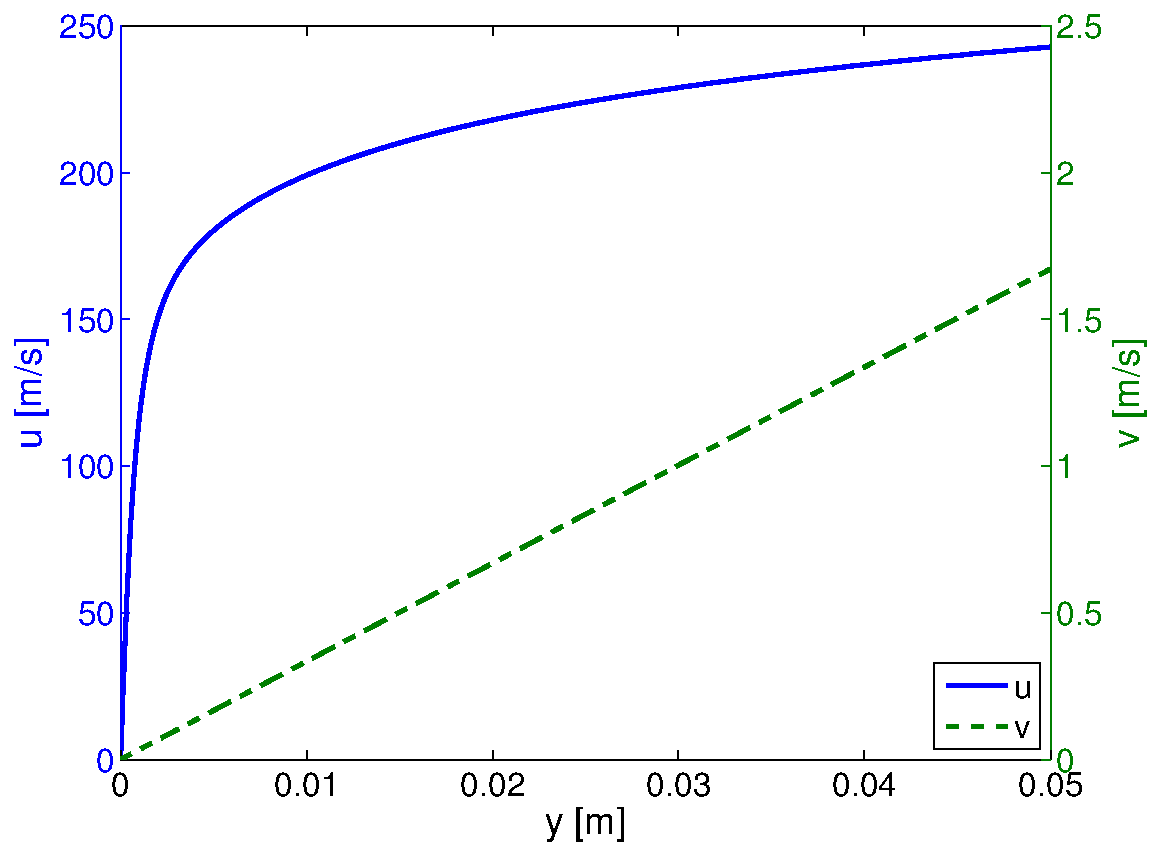
\includegraphics[width=0.5\linewidth]{figs/velocity_soln.pdf} \label{fig:velocity}}
\subfigure[The manufactured density and temperature profiles.]{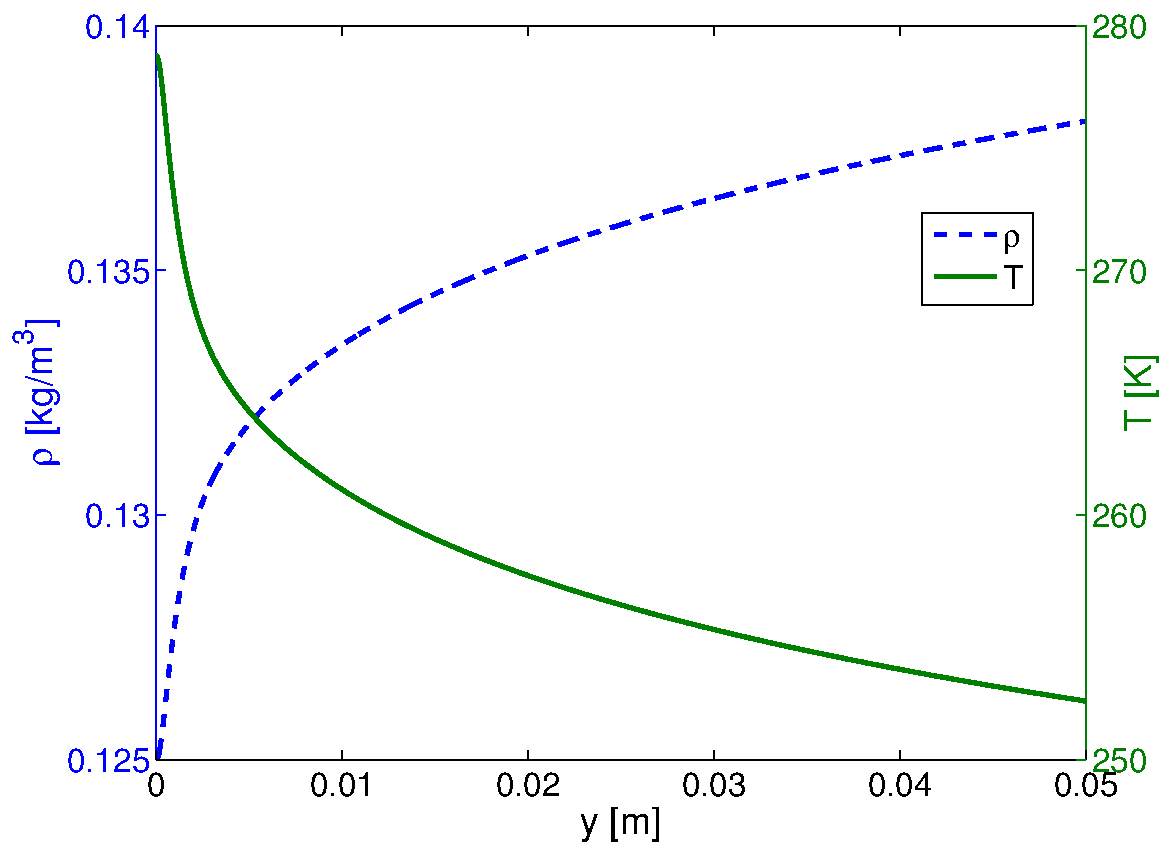
\includegraphics[width=0.5\linewidth]{figs/thermo_soln.pdf}\label{fig:thermo}}
\subfigure[The manufactured $\sa$ and $\chi$ profiles.]{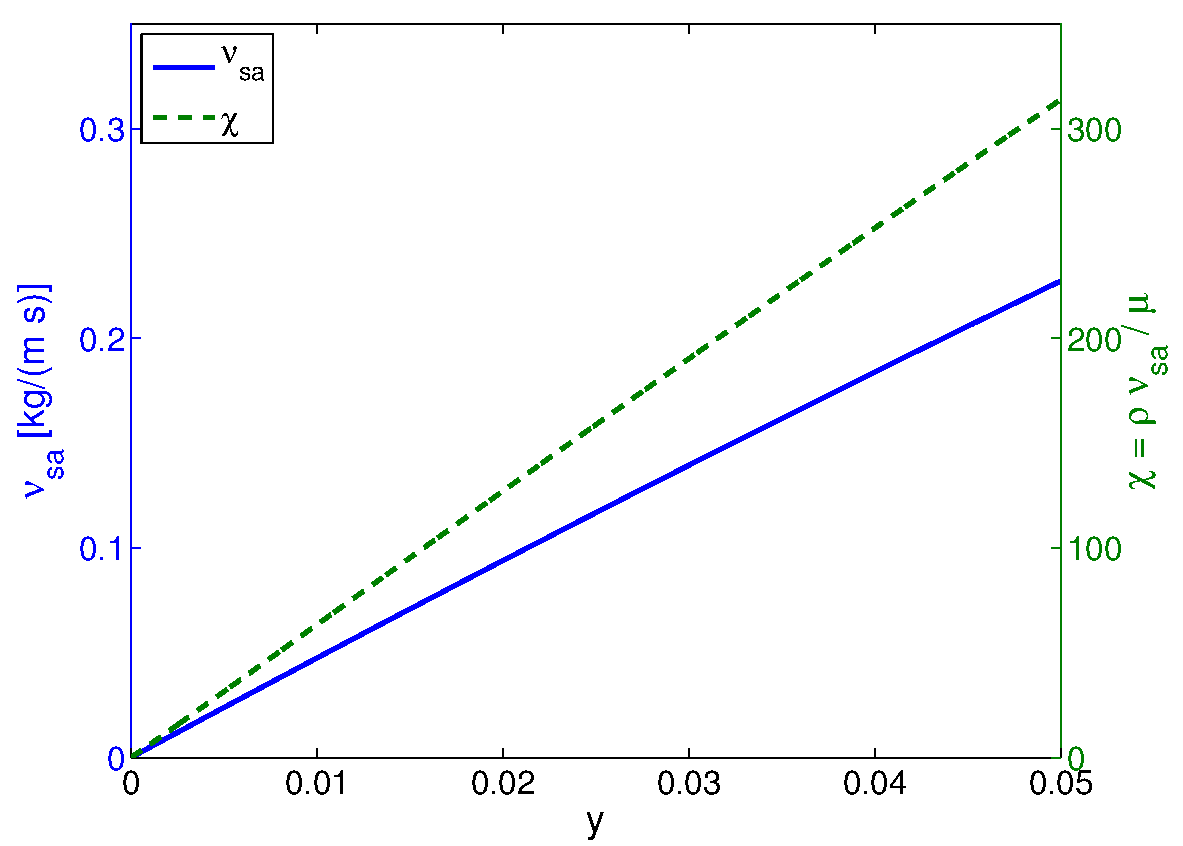
\includegraphics[width=0.5\linewidth]{figs/sa_var_soln.pdf} \label{fig:sa_profile}}
\end{center}
\vspace{-15pt}
\caption{Manufactured solutions profiles.}
\end{figure}

%
\section{SA Equation Budget} \label{sec:sa_budget}
The stated goal of this work is to develop a manufactured solution
that reasonably resembles a boundary layer.  This is most crucial with
respect to the turbulence model.  As demonstrated by \citet{Eca2007a}, the
observed behavior of the turbulence model can be highly sensitive to
the chosen manufactured solution.  To evaluate the current choices, we
plot the SA model equation budget.  The figures was generated using
the parameter values given in Section~\ref{sec:soln_plots}.  The curve
labeled ``Sum'' is equal to the sum of all of the SA terms collected
on the left hand side---i.e., it is the residual of the SA equation
evaluated at the manufactured state.  This residual is equivalent
to the source term that must be added to the right hand side to
balance the equation such that the manufactured state is a solution.
%
\begin{figure}[htp]

\begin{center}
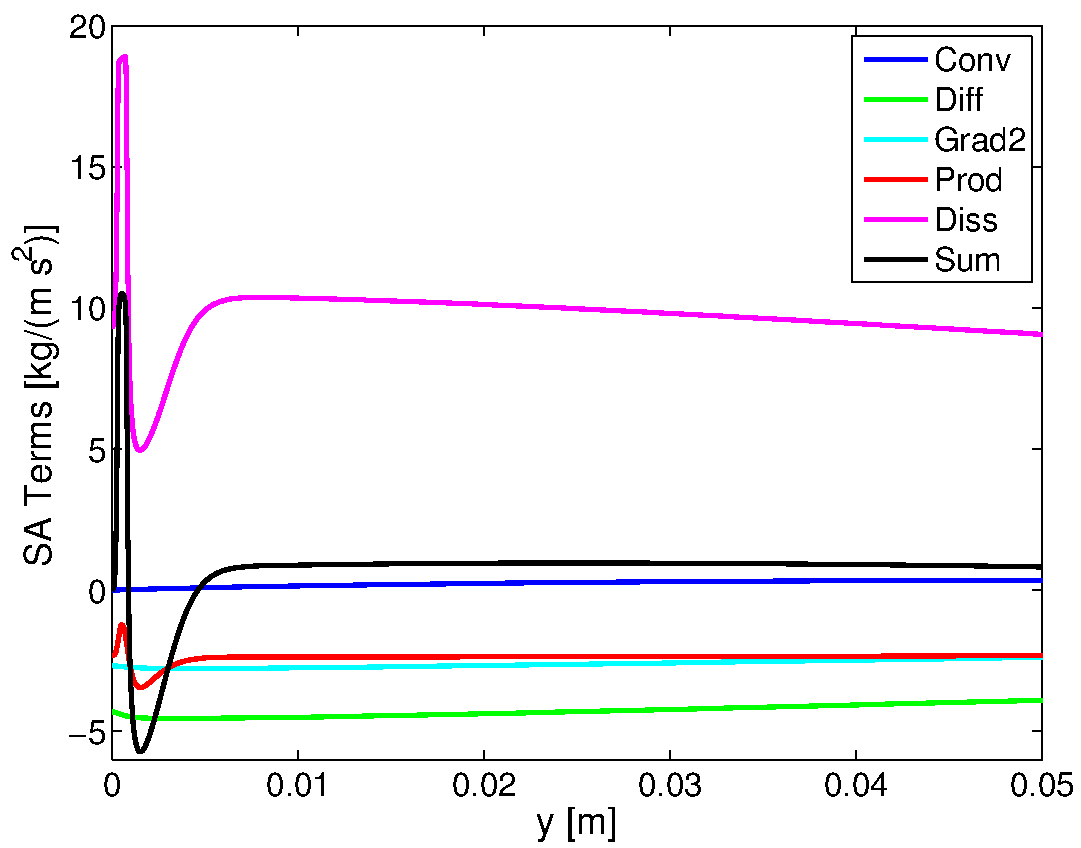
\includegraphics[width=0.5\linewidth]{figs/sa_budget.pdf}
\end{center}
\vspace{-15pt}
\caption{The Spalart-Allmaras model equation budget.}\label{fig:sa_budget}
\end{figure}

Figure \ref{fig:sa_budget} shows that for $y > 0.006 \, \mathrm{m} \approx 100
\ell_v$ the expected log layer behavior is roughly achieved.  All of
the SA terms except convection are significant and nearly in balance
(i.e., the residual term is significantly smaller than any of the
individual terms except convection).  For $y < 0.006 \,\mathrm{m}$,
the is residual is more significant, mostly due to the dissipation
term.  

Figure~\ref{fig:sa_budget_near_wall} shows the budget in this
region more clearly.
Very close to the wall ($0 \leq y \leq 1 \times 10^{-4} \approx 2
\ell_v$) the terms have the behavior expected in the viscous sublayer,
and the residual is small.  It appears that the large residual region
is associated with the transition from viscous sublayer behavior to
log layer behavior.  There is no reason to expect that the
manufactured solution constructed in this work is close to the true SA
model solution in this region.  Thus, it is reasonable for the SA
equation to be more out of balance, leading to the
larger residual in this region.
%
\begin{figure}[htp]
\begin{center}
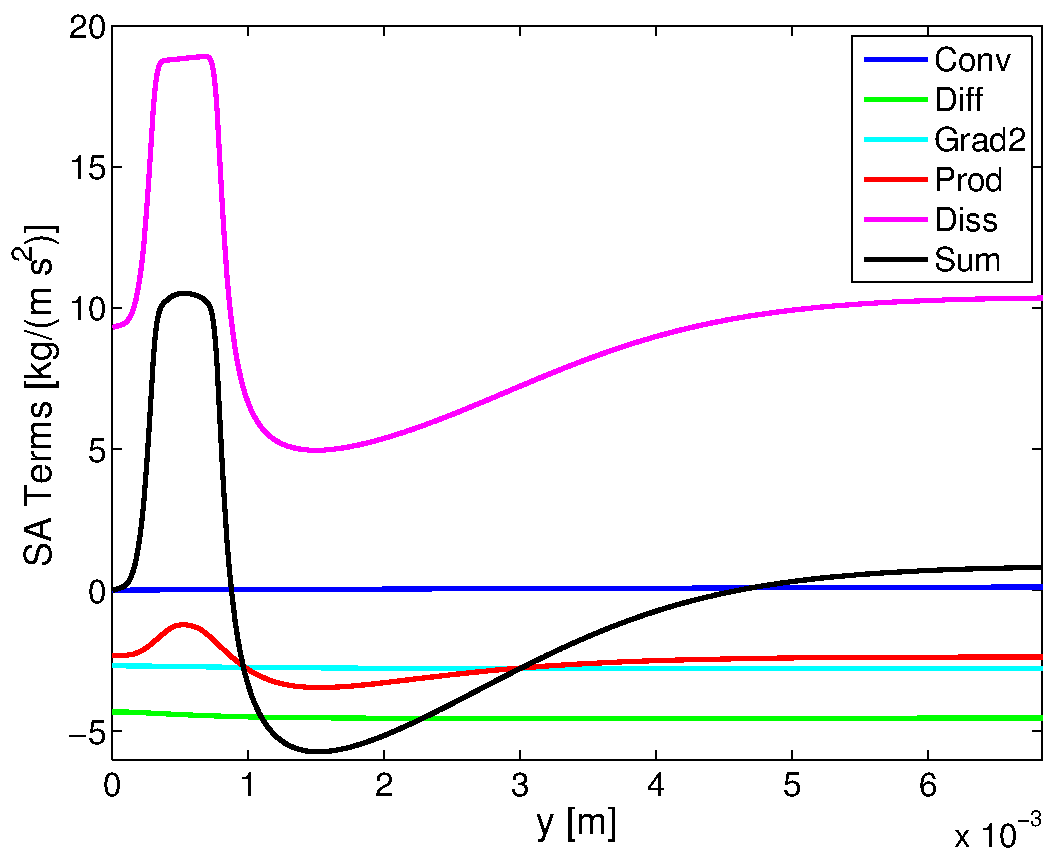
\includegraphics[width=0.5\linewidth]{figs/sa_budget_near_wall.pdf}
\end{center}
\vspace{-15pt}
\caption{The Spalart-Allmaras model equation budget very close to the wall ($0 \leq y \leq 100 \ell_v$).}\label{fig:sa_budget_near_wall}
\end{figure}
% 
%\section{List of constants}

There are a variety of constants present in the FANS-SA formulation due to both fluid properties and SA calibration. The total amount is further increased due to the constants arising from the chosen manufactured solutions.

\begin{description}
	\item[Fluid properties:] $\mu, \,c_v, \, c_p,\,p_0$.

\item[SA calibration model:] $\sigma, \, \kappa, \, c_{b1}, \, c_{b2}, \, c_{v1}, \, c_{v2}, \, c_{v3}, \, c_{w1}, \, c_{w2}, \, c_{w3}$.

\item[Manufactured solutions:] $u_\infty, \, A, \, \eta_v, \, T_\infty, \, T_{aw},\, M_\infty, \, r_T,$  $\gamma, %\, \kappa (again, ask Todd), \,
\alpha, \, C_{cf}, \, F_c, \, \rho_\infty, \, C_1, \, C,\, \eta_1, \, b, \, \nu_w$.

Additionally, 


$$C_1=-\dfrac{1}{\kappa} \log(\kappa)+C,$$%\quad \text{with}\quad C \text{ constant,}$$
$$T_{aw} =  T_{\infty} \left[ 1 + r_T \frac{\gamma - 1}{2} M_{\infty}^2 \right],$$
$$A = \sqrt{1 - T_{\infty}/T_{aw}},$$
$$ F_c = \frac{T_{aw}/T_{\infty} - 1}{ \left( \sin^{-1} A \right)^2} .$$
\end{description}




\end{document}

@Article{ ISI:000285551800008,
	Author = "Kevin Long and Robert Kirby and Bart Van Bloemen Waanders",
	Title = "{UNIFIED EMBEDDED PARALLEL FINITE ELEMENT COMPUTATIONS VIA SOFTWARE-BASED FRECHET DIFFERENTIATION}",
	Journal = "{SIAM JOURNAL ON SCIENTIFIC COMPUTING}",
	Year = "{2010}",
	Volume = "{32}",
	Number = "{6}",
	Pages = "{3323--3351}",
	Abstract = "{Computational analysis of systems governed by partial differential equations (PDEs) requires not only the calculation of a solution but the extraction of additional information such as the sensitivity of that solution with respect to input parameters or the inversion of the system in an optimization or design loop. Moving beyond the automation of discretization of PDEs by finite element methods, we present a mathematical framework that unifies the discretization of PDEs with these additional analysis requirements. In particular, Frechet differentiation on a class of functionals together with a high-performance finite element framework has led to a code, called Sundance, that provides high-level programming abstractions for the automatic, efficient evaluation of finite variational forms together with the derived operators required by engineering analysis.}",
	Publisher = "{SIAM PUBLICATIONS}",
	Address = "{3600 UNIV CITY SCIENCE CENTER, PHILADELPHIA, PA 19104-2688 USA}",
	Type = "{Article}",
	Language = "{English}",
	Affiliation = "{Long, K (Reprint Author), Texas Tech Univ, Dept Math \& Stat, Lubbock, TX 79409 USA. {[}Long, Kevin; Kirby, Robert] Texas Tech Univ, Dept Math \& Stat, Lubbock, TX 79409 USA. {[}Waanders, Bart Van Bloemen] Sandia Natl Labs, Albuquerque, NM 87122 USA.}",
	DOI = "{10.1137/09076920X}",
	ISSN = "{1064-8275}",
	Keywords = "{finite element method, partial differential equations, embedded algorithms}",
	Keywords-Plus = "{VARIATIONAL FORMS; MATRICES; CODE; OPTIMIZATION; VERIFICATION; GENERATION; TRANSFORMS; FLAME}",
	Subject-Category = "{Mathematics, Applied}",
	Author-Email = "{kevin.long@ttu.edu robert.c.kirby@ttu.edu bartv@sandia.gov}",
	Funding-Acknowledgement = "{U.S. Department of Energy {[}DE-AC04-94AL85000]}",
	Funding-Text = "{Applied Mathematics and Applications, Sandia National Laboratories, P.O. Box 5800, Albuquerque, NM 87122 (bartv@sandia.gov). Sandia is a multiprogram laboratory operated by Sandia Corporation, a Lockheed Martin company, for the U.S. Department of Energy under contract DE-AC04-94AL85000.}",
	Number-of-Cited-References = "{43}",
	Times-Cited = "{0}",
	Journal-ISO = "{SIAM J. Sci. Comput.}",
	Doc-Delivery-Number = "{697WZ}",
	Unique-ID = "{ISI:000285551800008}"
}
\begin{equation}
	\begin{split}
\diff{T}{x} &= -\dfrac{1}{14} \dfrac{r_T\, (\gamma-1)\, M_{\infty}^2 \,T_{\infty}\, u_\tau \, }{u_{\infty}^2 x}\, u \,\cos\left(\dfrac{A u_{eq}}{u_{\infty}}\right) \left[y^{+} \Dueqplusyplus+u_{eq}^{+}\right]\\
%
\diff{T}{y} &=  \dfrac{r_T\, (\gamma-1)\, M_{\infty}^2 \,T_{\infty}\,  u_\tau\,  y^{+} }{u_{\infty}^2 y}\, u \,\cos\left(\dfrac{A u_{eq}}{u_{\infty}}\right)  \Dueqplusyplus\\
%
\diff{ u}{x} &= -\dfrac{1}{14}\dfrac{u_\tau }{x}\cos\left(\dfrac{A u_{eq}}{u_{\infty}}\right) \left[y^{+} \Dueqplusyplus+u_{eq}^{+}\right]\\
\diff{ u}{y} &= y^{+} \dfrac{ u_\tau }{y} \Dueqplusyplus \cos\left(\dfrac{A u_{eq}}{u_{\infty}}\right)\\
\diff{ v}{x} &= -\dfrac{15}{196}\dfrac{ \eta_v u_\tau y}{x^2}\\
\diff{ v}{y} &= \dfrac{1}{14}\dfrac{\eta_v u_\tau}{x}\\
\diff{ \sa}{x} &= -\dfrac{1}{14}\dfrac{ \kappa u_\tau y}{x}\\
\diff{\sa}{y} &= \kappa u_\tau-2 \alpha y\\
\diff{\rho}{x} &= \dfrac{1}{14}\dfrac{p_0}{R T^2} \dfrac{r_T\, (\gamma-1)\, M_{\infty}^2 \,T_{\infty}\, u_\tau \, }{u_{\infty}^2 x}\, u \,\cos\left(\dfrac{A u_{eq}}{u_{\infty}}\right) \left[y^{+} \Dueqplusyplus+u_{eq}^{+}\right]\\
\diff{\rho}{y} &=- \dfrac{p_0}{R T^2}  \dfrac{r_T\, (\gamma-1)\, M_{\infty}^2 \,T_{\infty}\,  u_\tau\, y^{+}}{u_{\infty}^2 y}\, u \,\cos\left(\dfrac{A u_{eq}}{u_{\infty}}\right)   \Dueqplusyplus
%		
\end{split}
\end{equation}